\documentclass[10pt]{beamer}

\usetheme[progressbar=frametitle]{metropolis}
\usepackage{appendixnumberbeamer}

\usepackage{amsfonts}
\usepackage{amssymb}
\usepackage{amsthm}
\usepackage{amsmath}
\usepackage{amsopn} 
\usepackage{multimedia}
\usepackage{media9}
\usepackage{caption}
\usepackage{multicol}
\graphicspath{{figures/}}

\usepackage{wrapfig}

\usepackage{booktabs}
\usepackage[scale=2]{ccicons}

\usepackage{pgfplots}
\usepgfplotslibrary{dateplot}

\usepackage{xspace}
\newcommand{\themename}{\textbf{\textsc{metropolis}}\xspace}

\title{Optimising the thickness determination of homopolymers and diblock copolymers using optical spectral reflectance during solvent vapour annealing}
\subtitle{INM - RUC 2019 - Master's Thesis \\ Supervisor: Dorthe Posselt}
\date{7/5/2019}
\author{Nathan Hugh Barr}
\institute{Roskilde University}

\begin{document}

\maketitle

\begin{frame}{Tabel of contents}
\begin{multicols}{2}
\setbeamertemplate{section in toc}[sections numbered]
\tableofcontents[hideallsubsections]
\end{multicols}
\end{frame}

%\begin{frame}{Table of contents}
%  \setbeamertemplate{section in toc}[sections numbered]
%  \tableofcontents[hideallsubsections]
%\end{frame}

	\section{Master Thesis Prelude}

%\begin{frame}{Cornell High Energy Synchrotron Source (CHESS)}
%	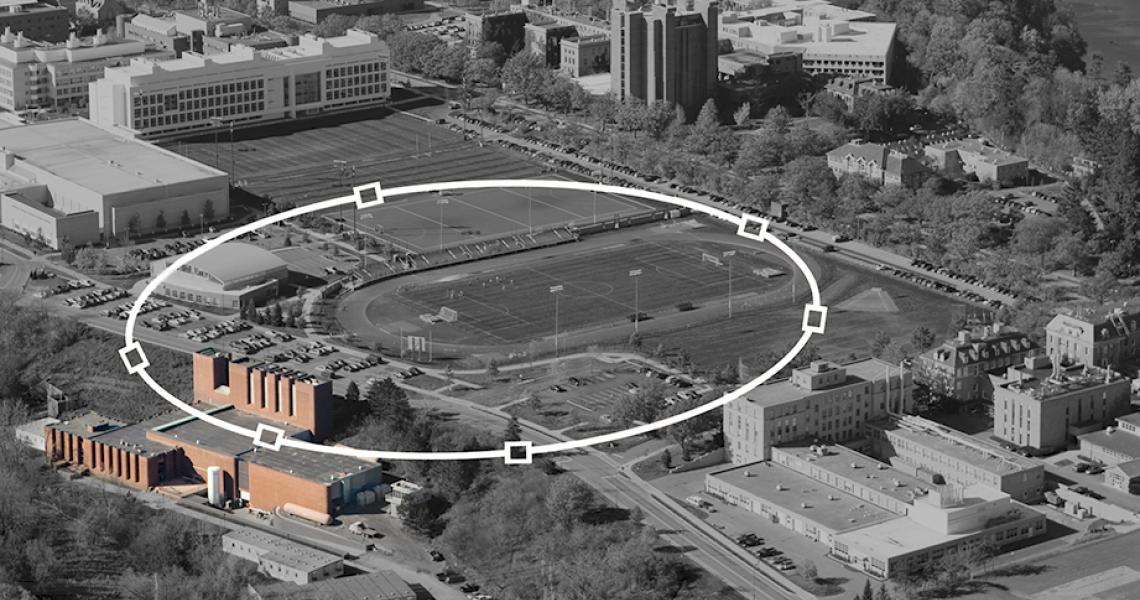
\includegraphics[width=\textwidth]{Ring.jpg}
%\end{frame}

\begin{frame}{D-Line}
December '17 and May '18
	\begin{figure}
		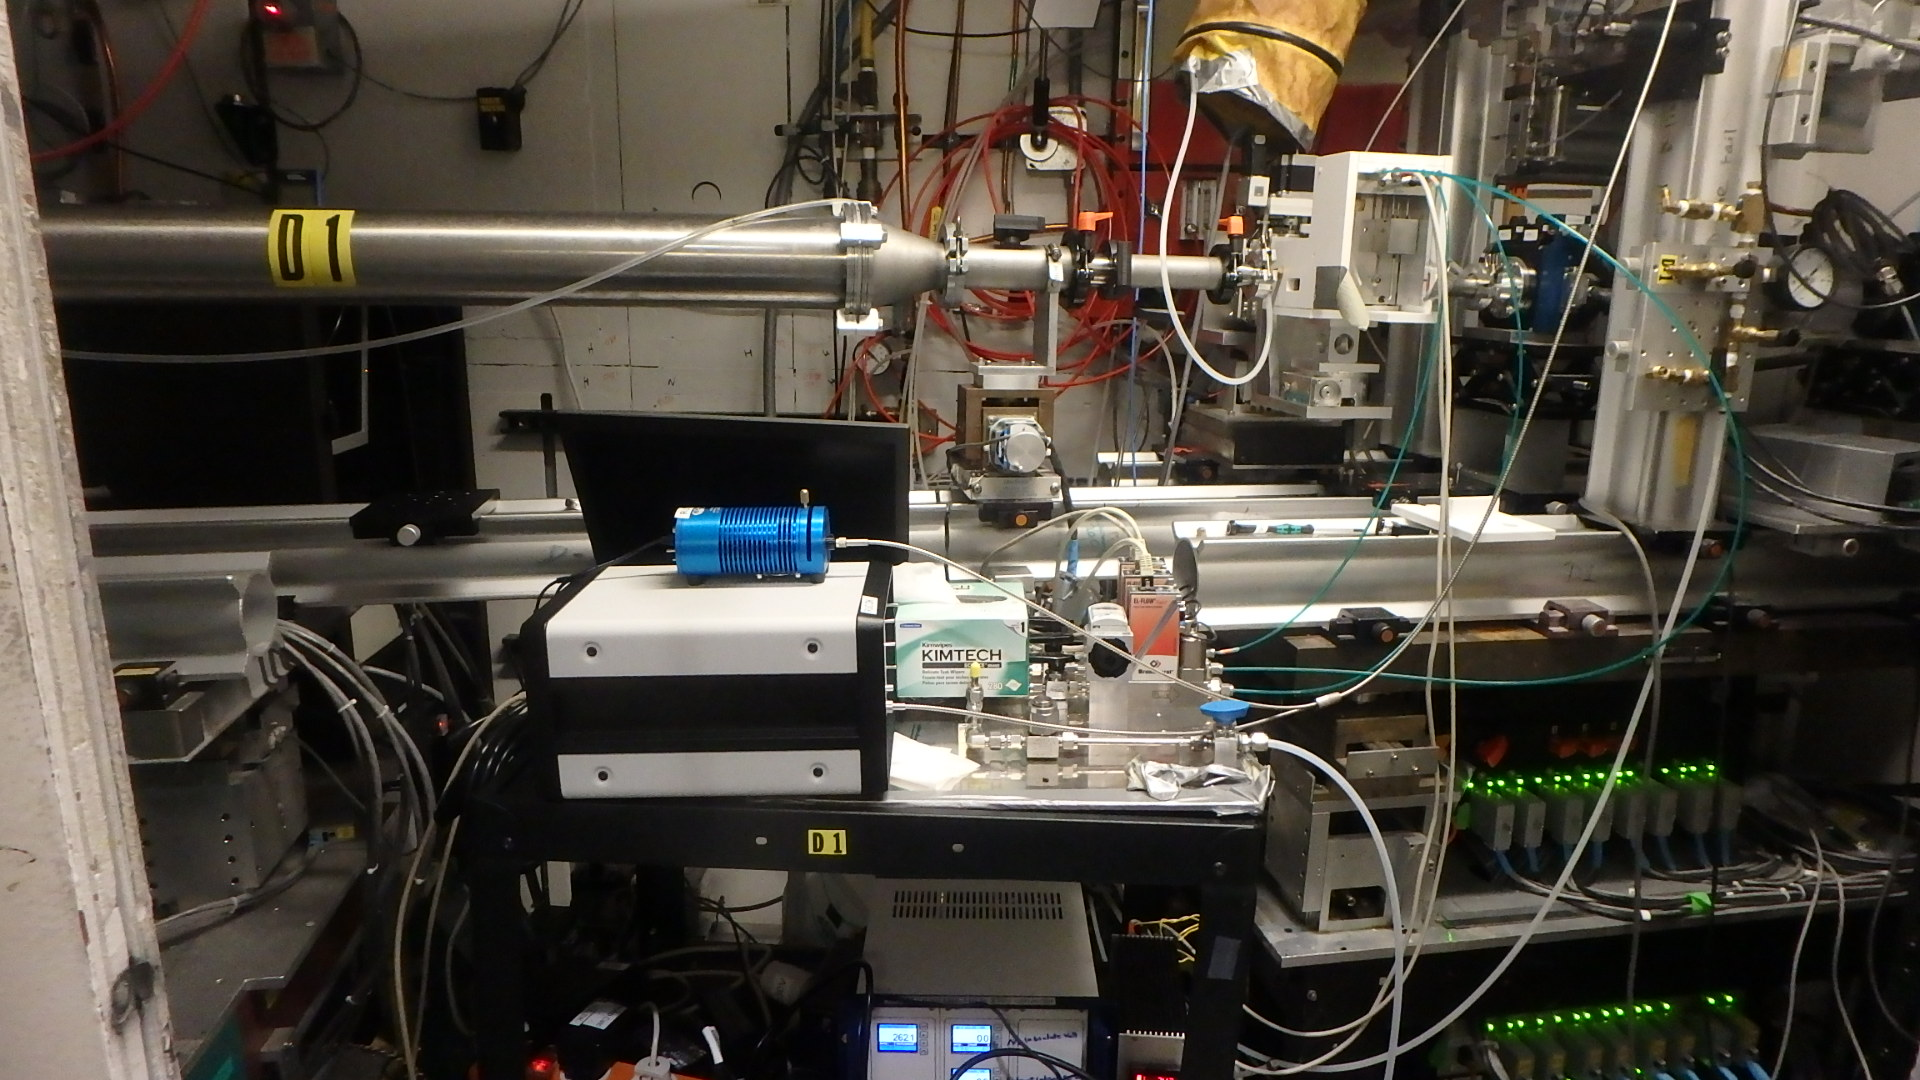
\includegraphics[scale=0.15]{chess3.JPG}
	\end{figure}
\end{frame}

\begin{frame}{Problems with the reflectance measurements during swelling}
	\centering
	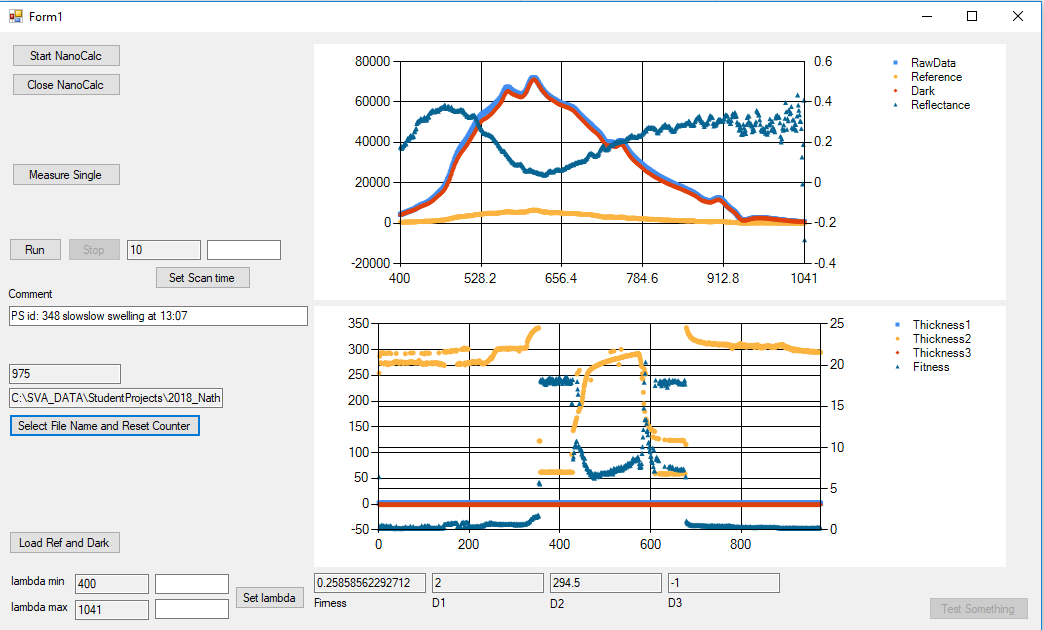
\includegraphics[height=0.35\textheight]{badmeasure2.png}
	\captionof{figure}{Polystyrene - SVA run used in Master Thesis}
	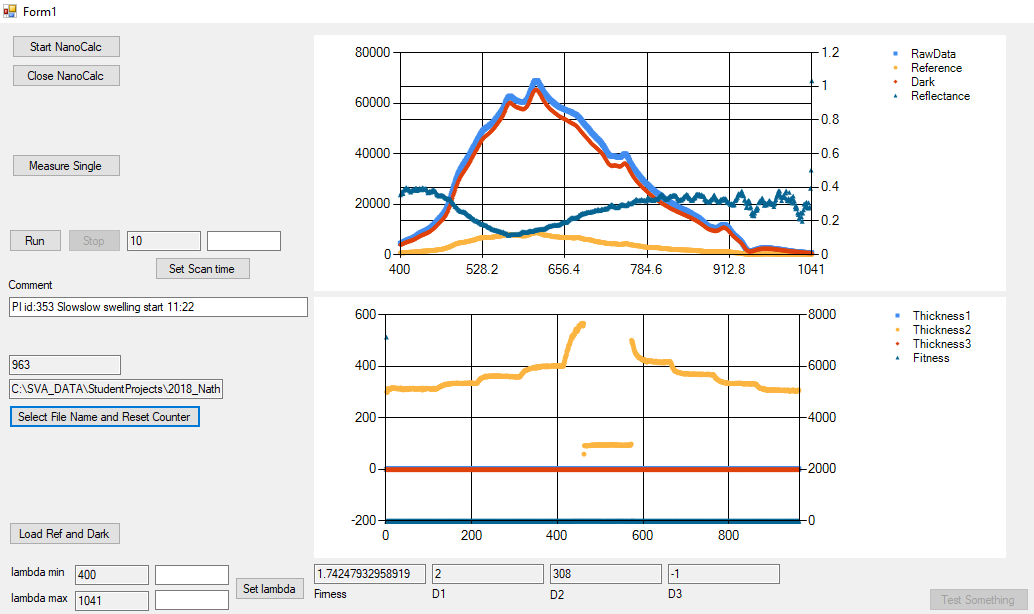
\includegraphics[height=0.35\textheight]{badmeasure3.png}
	\captionof{figure}{Polyisoprene - SVA run used in Master Thesis}
\end{frame}


	\section{Master Thesis Problem Formulation}


\begin{frame}{Problem Formulation}
What are the advantages and limitations when using optical spectral reflectance for determining the thickness of thin polymer films during solvent vapour annealing?

What is the optimal modelling and fitting method for the optical spectral reflectance measurements and thickness determination of the homopolymers, polystyrene and polyisoprene thin films during solvent vapour annealing?  
		
Can the same thickness determination be used on thin films with a horizontal nano scale structure such as the diblock-copolymer Polystyrene-b-Polyisoprene? 
\end{frame}
	
	
	\section{Experimental Setup}
	
\begin{frame}{Experimental Setup Overview}
	\begin{figure}
	\centering
	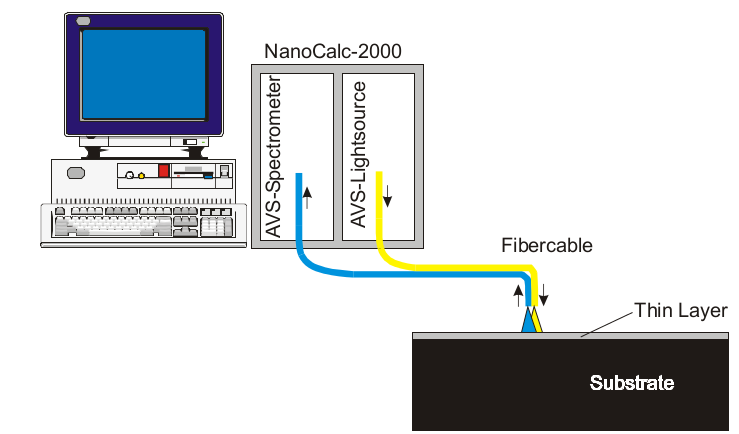
\includegraphics[width=\textwidth]{nanocalcsetup.png}
	\caption{Taken from NanoCalc Software Manual v.4}
	\end{figure}
\end{frame}	
		
%\begin{frame}{Experimental Components}
%NanoCalc XR, Halogen Light Source, Test Chamber and Single Point Stage
%		
%\begin{minipage}{0.47\textwidth}
%\begin{figure}
%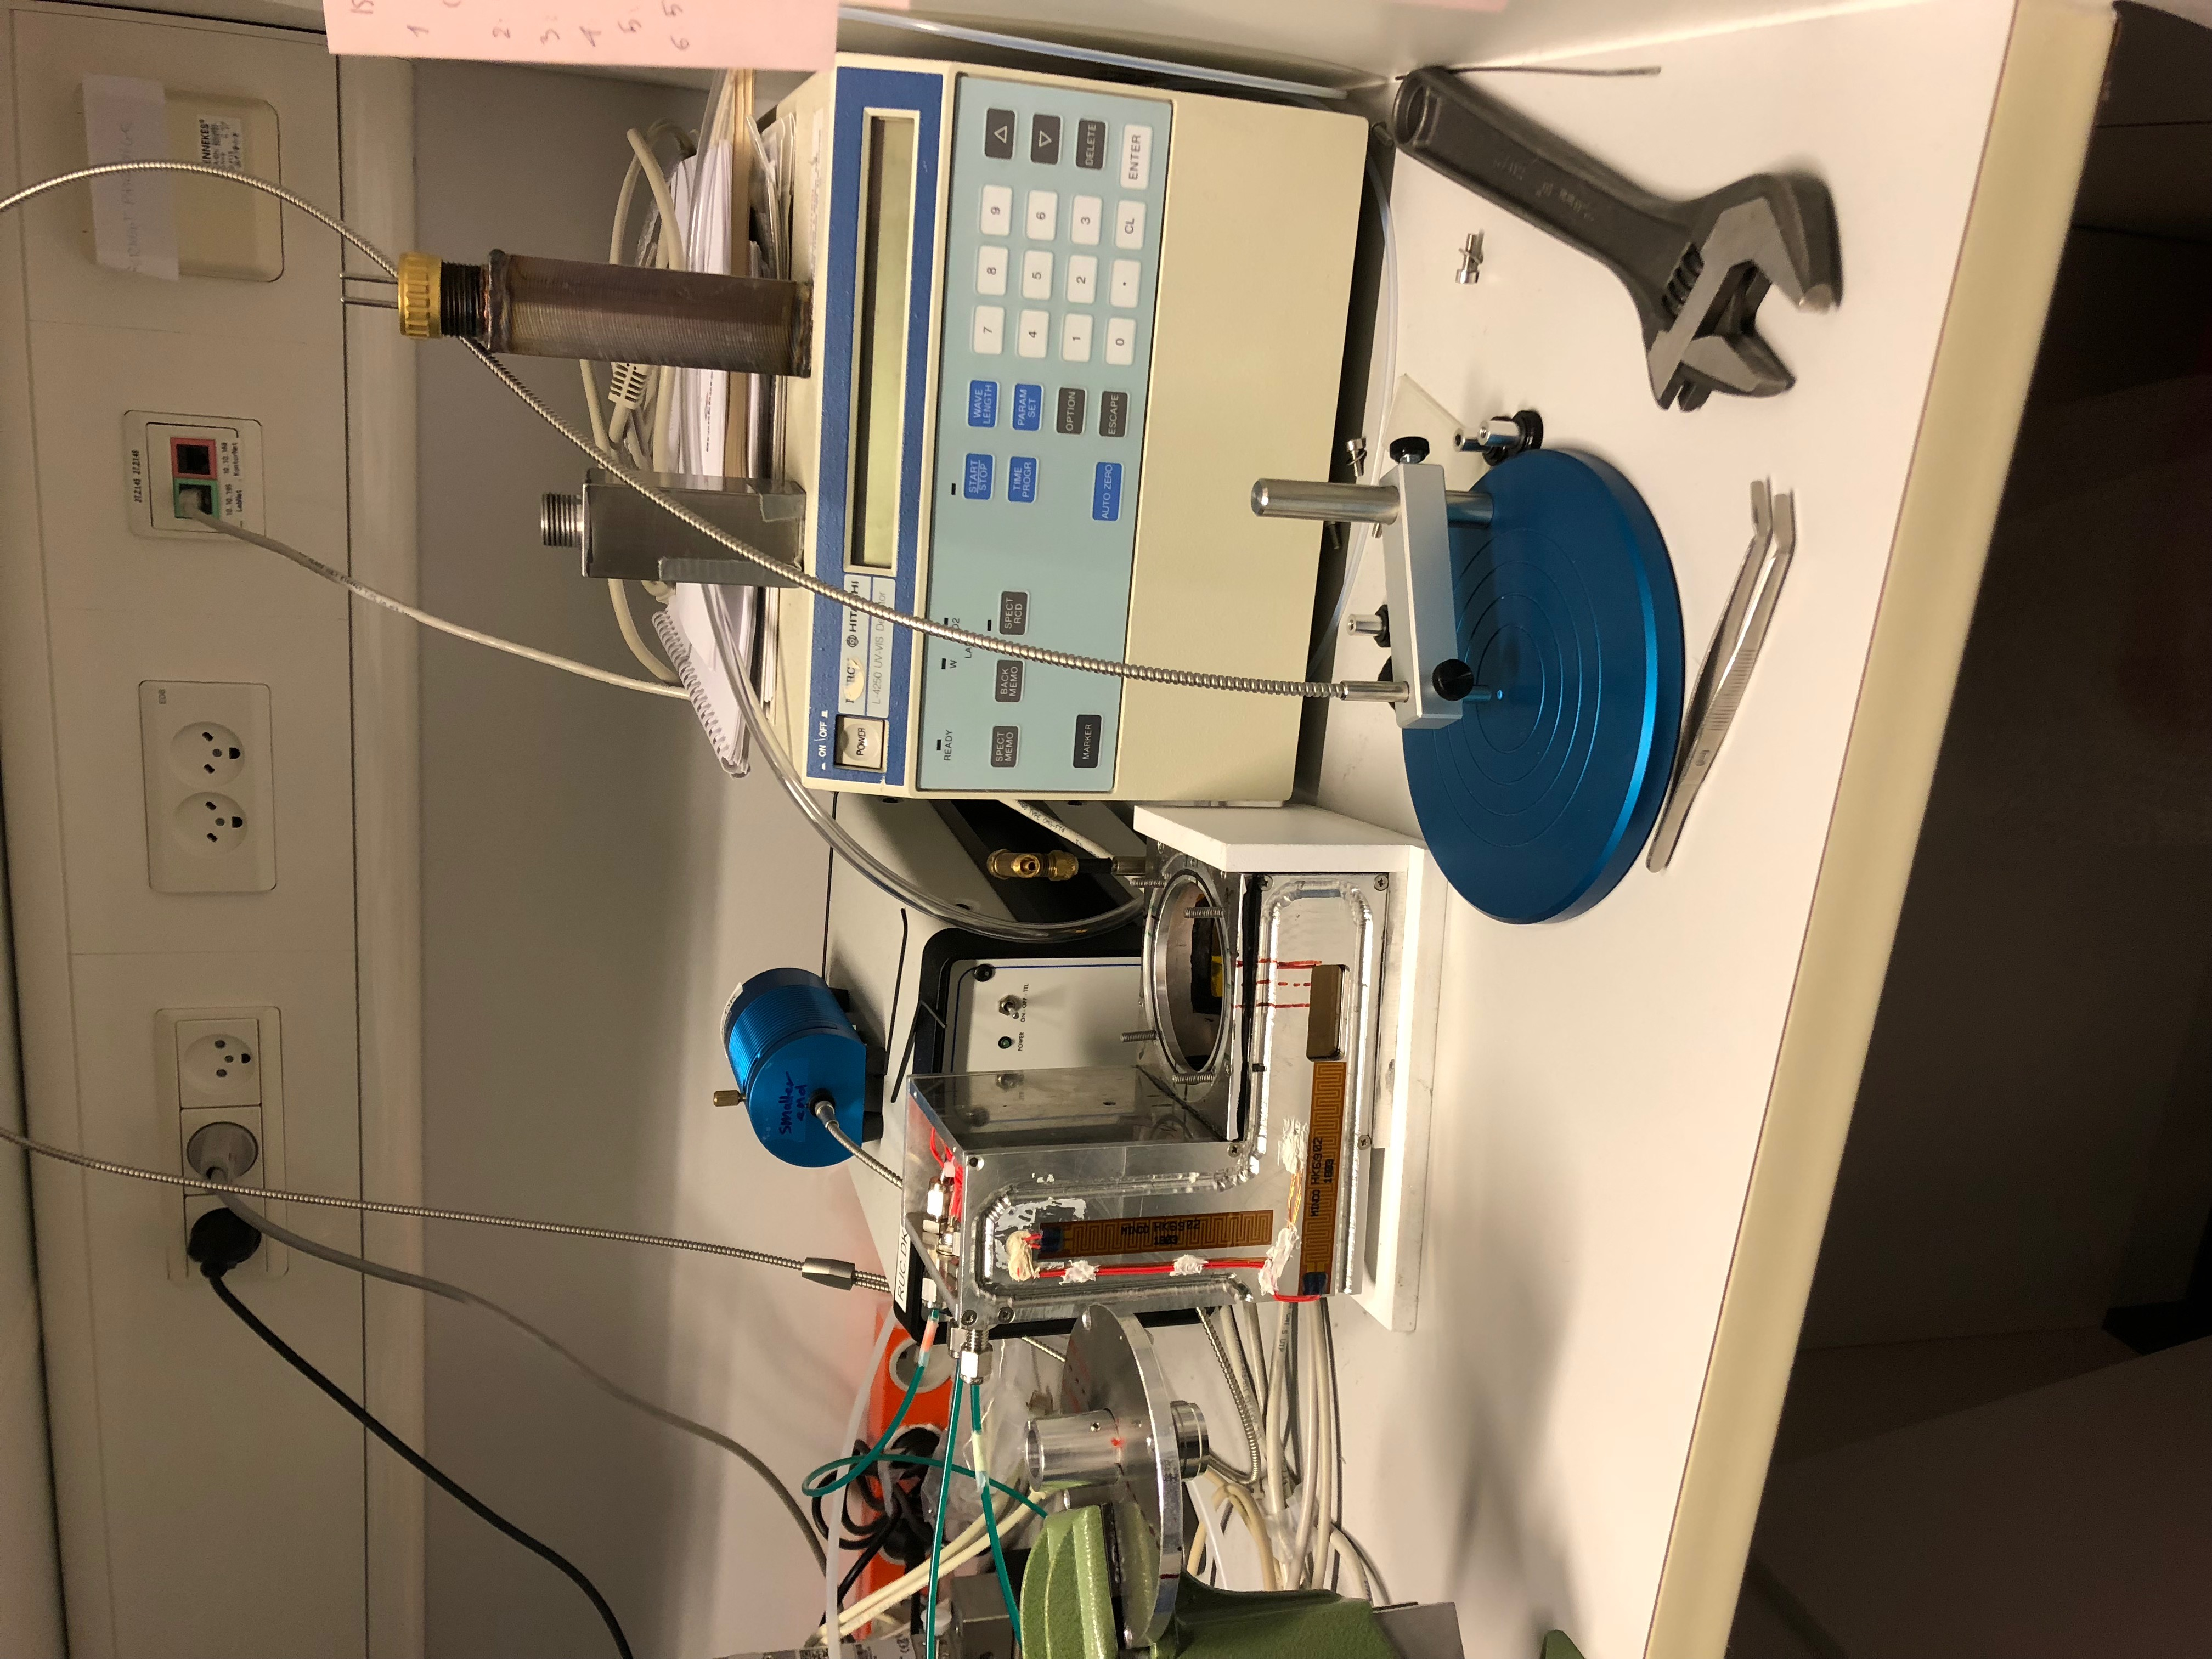
\includegraphics[scale=0.04,angle=-90]{setup1.JPG}
%\end{figure}
%\end{minipage}
%\begin{minipage}{0.5\textwidth}
%\begin{figure}
%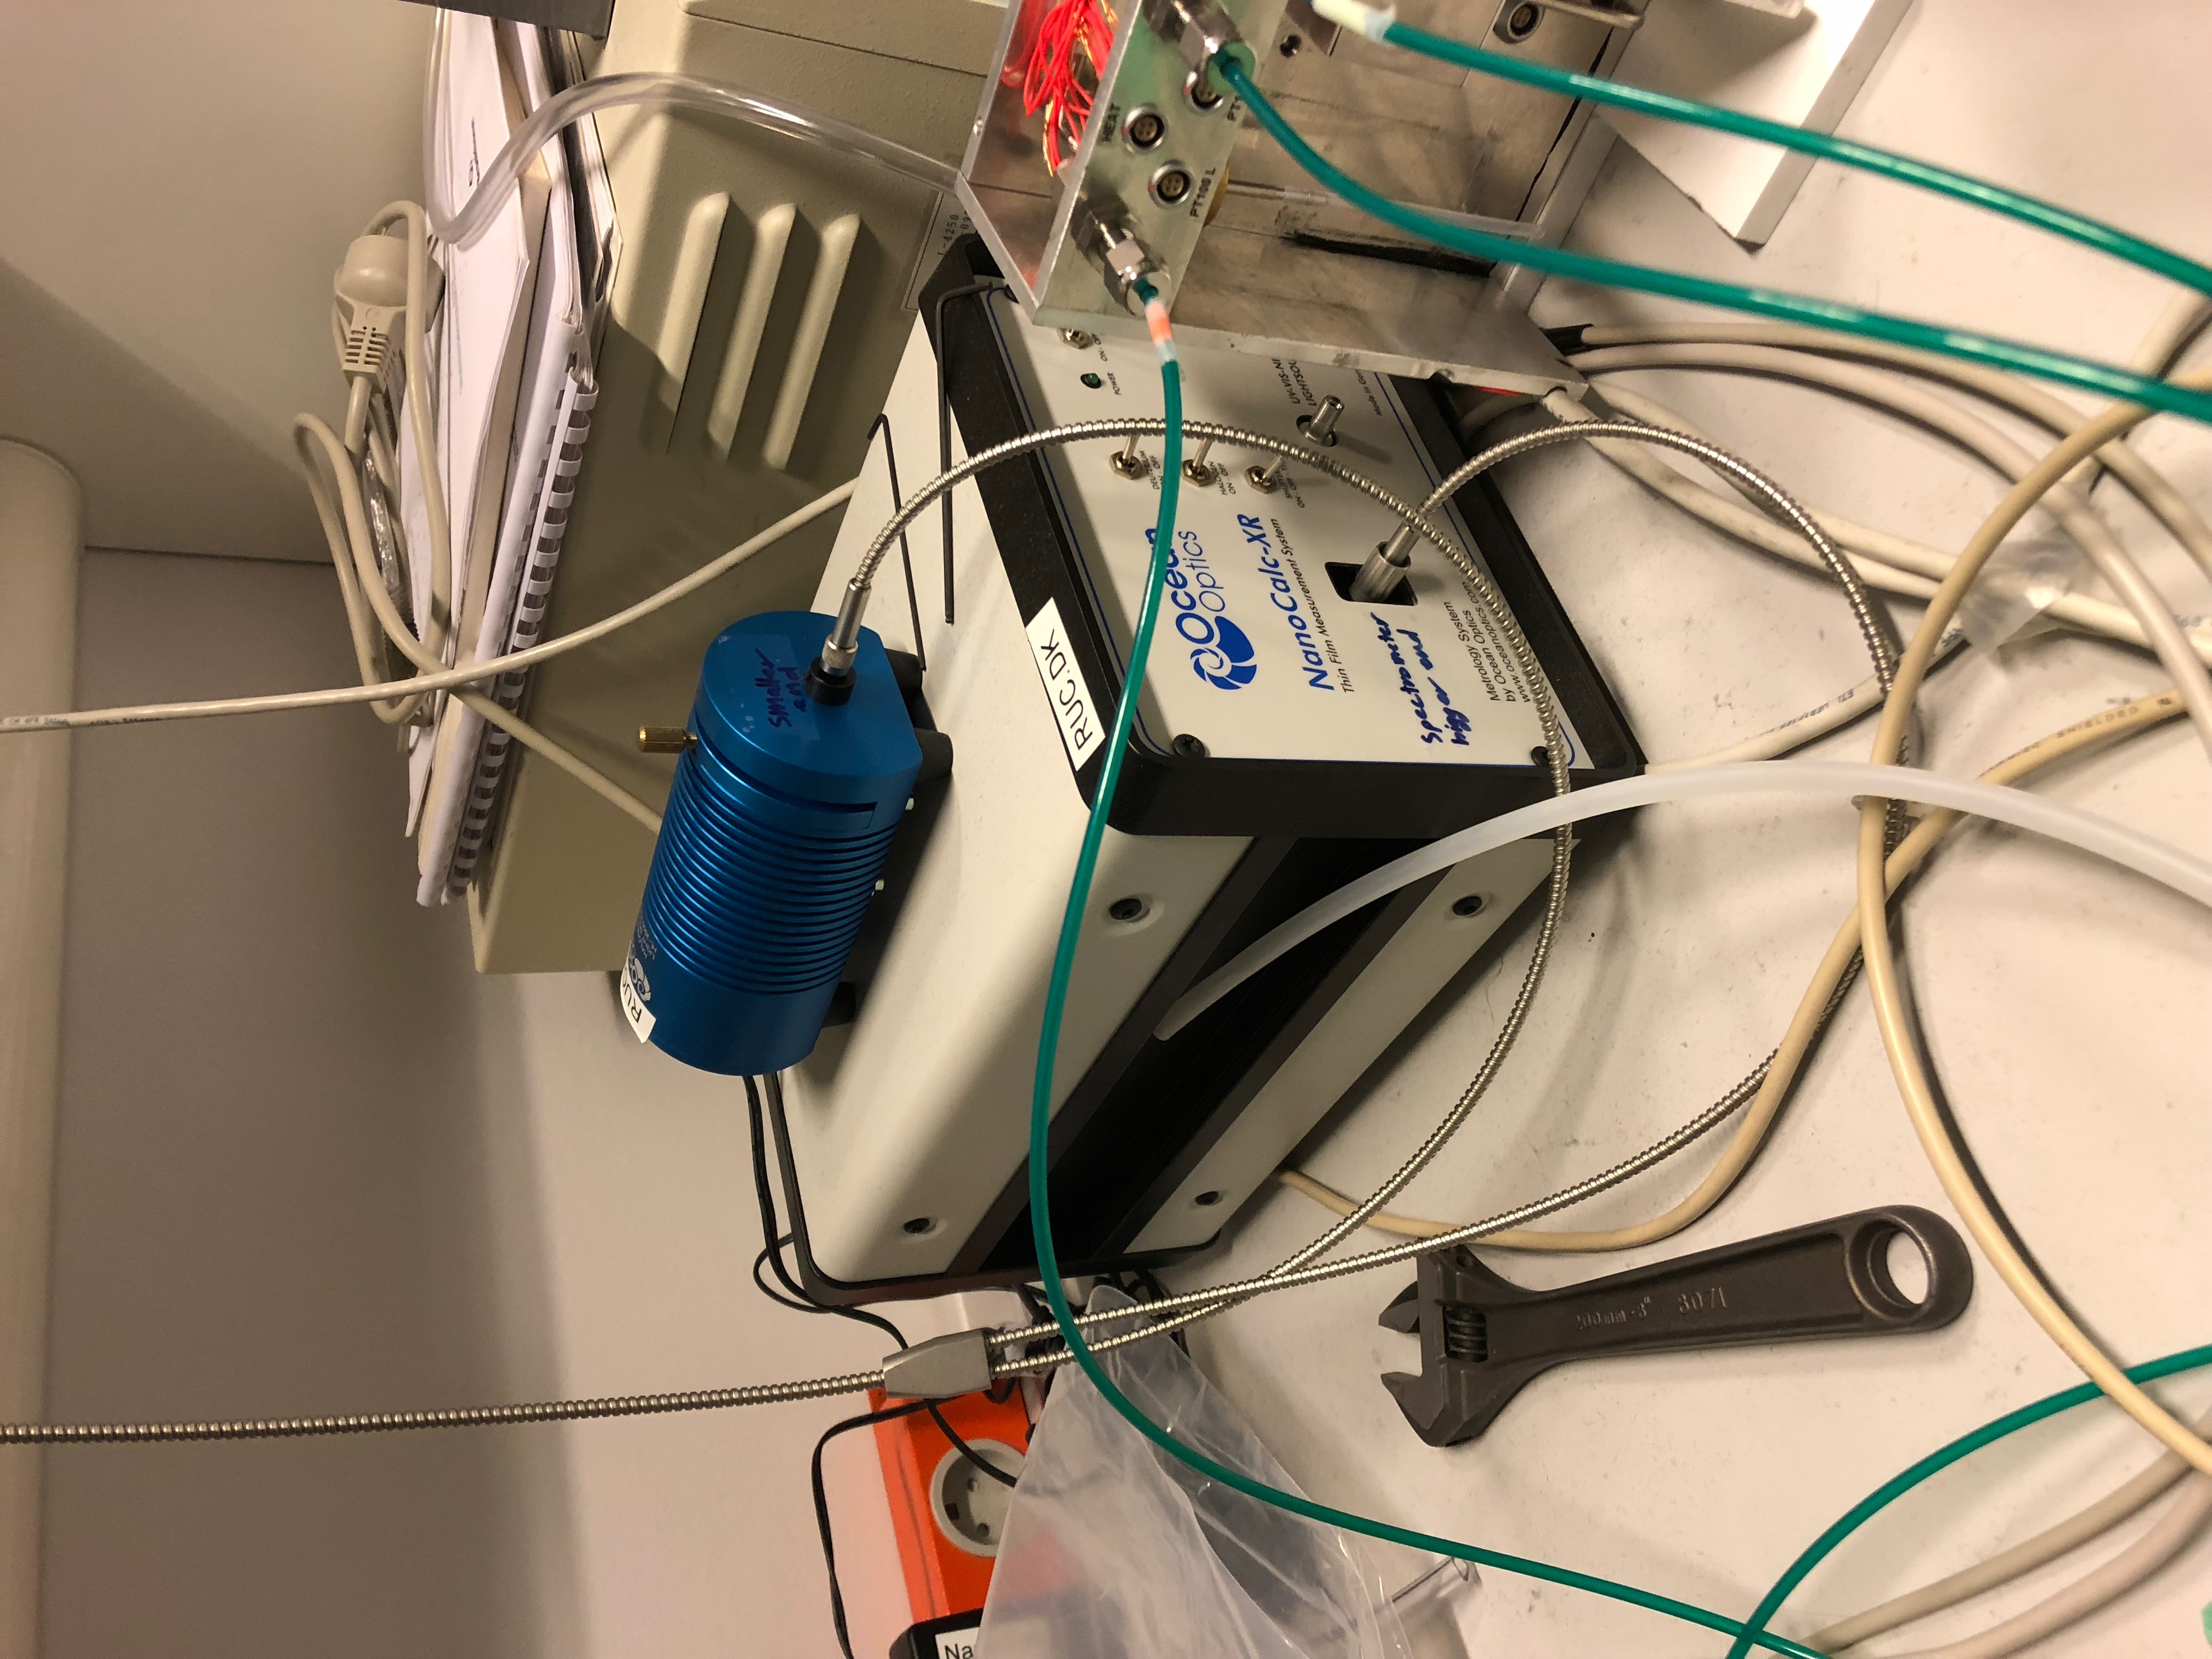
\includegraphics[scale=0.04,angle=-90]{setup2.JPG}
%\end{figure}
%\end{minipage}
%	
%\end{frame}

\begin{frame}{Experimental Components}
Single Point Stage and SVA test chamber.
\begin{minipage}{0.47\textwidth}
\begin{figure}
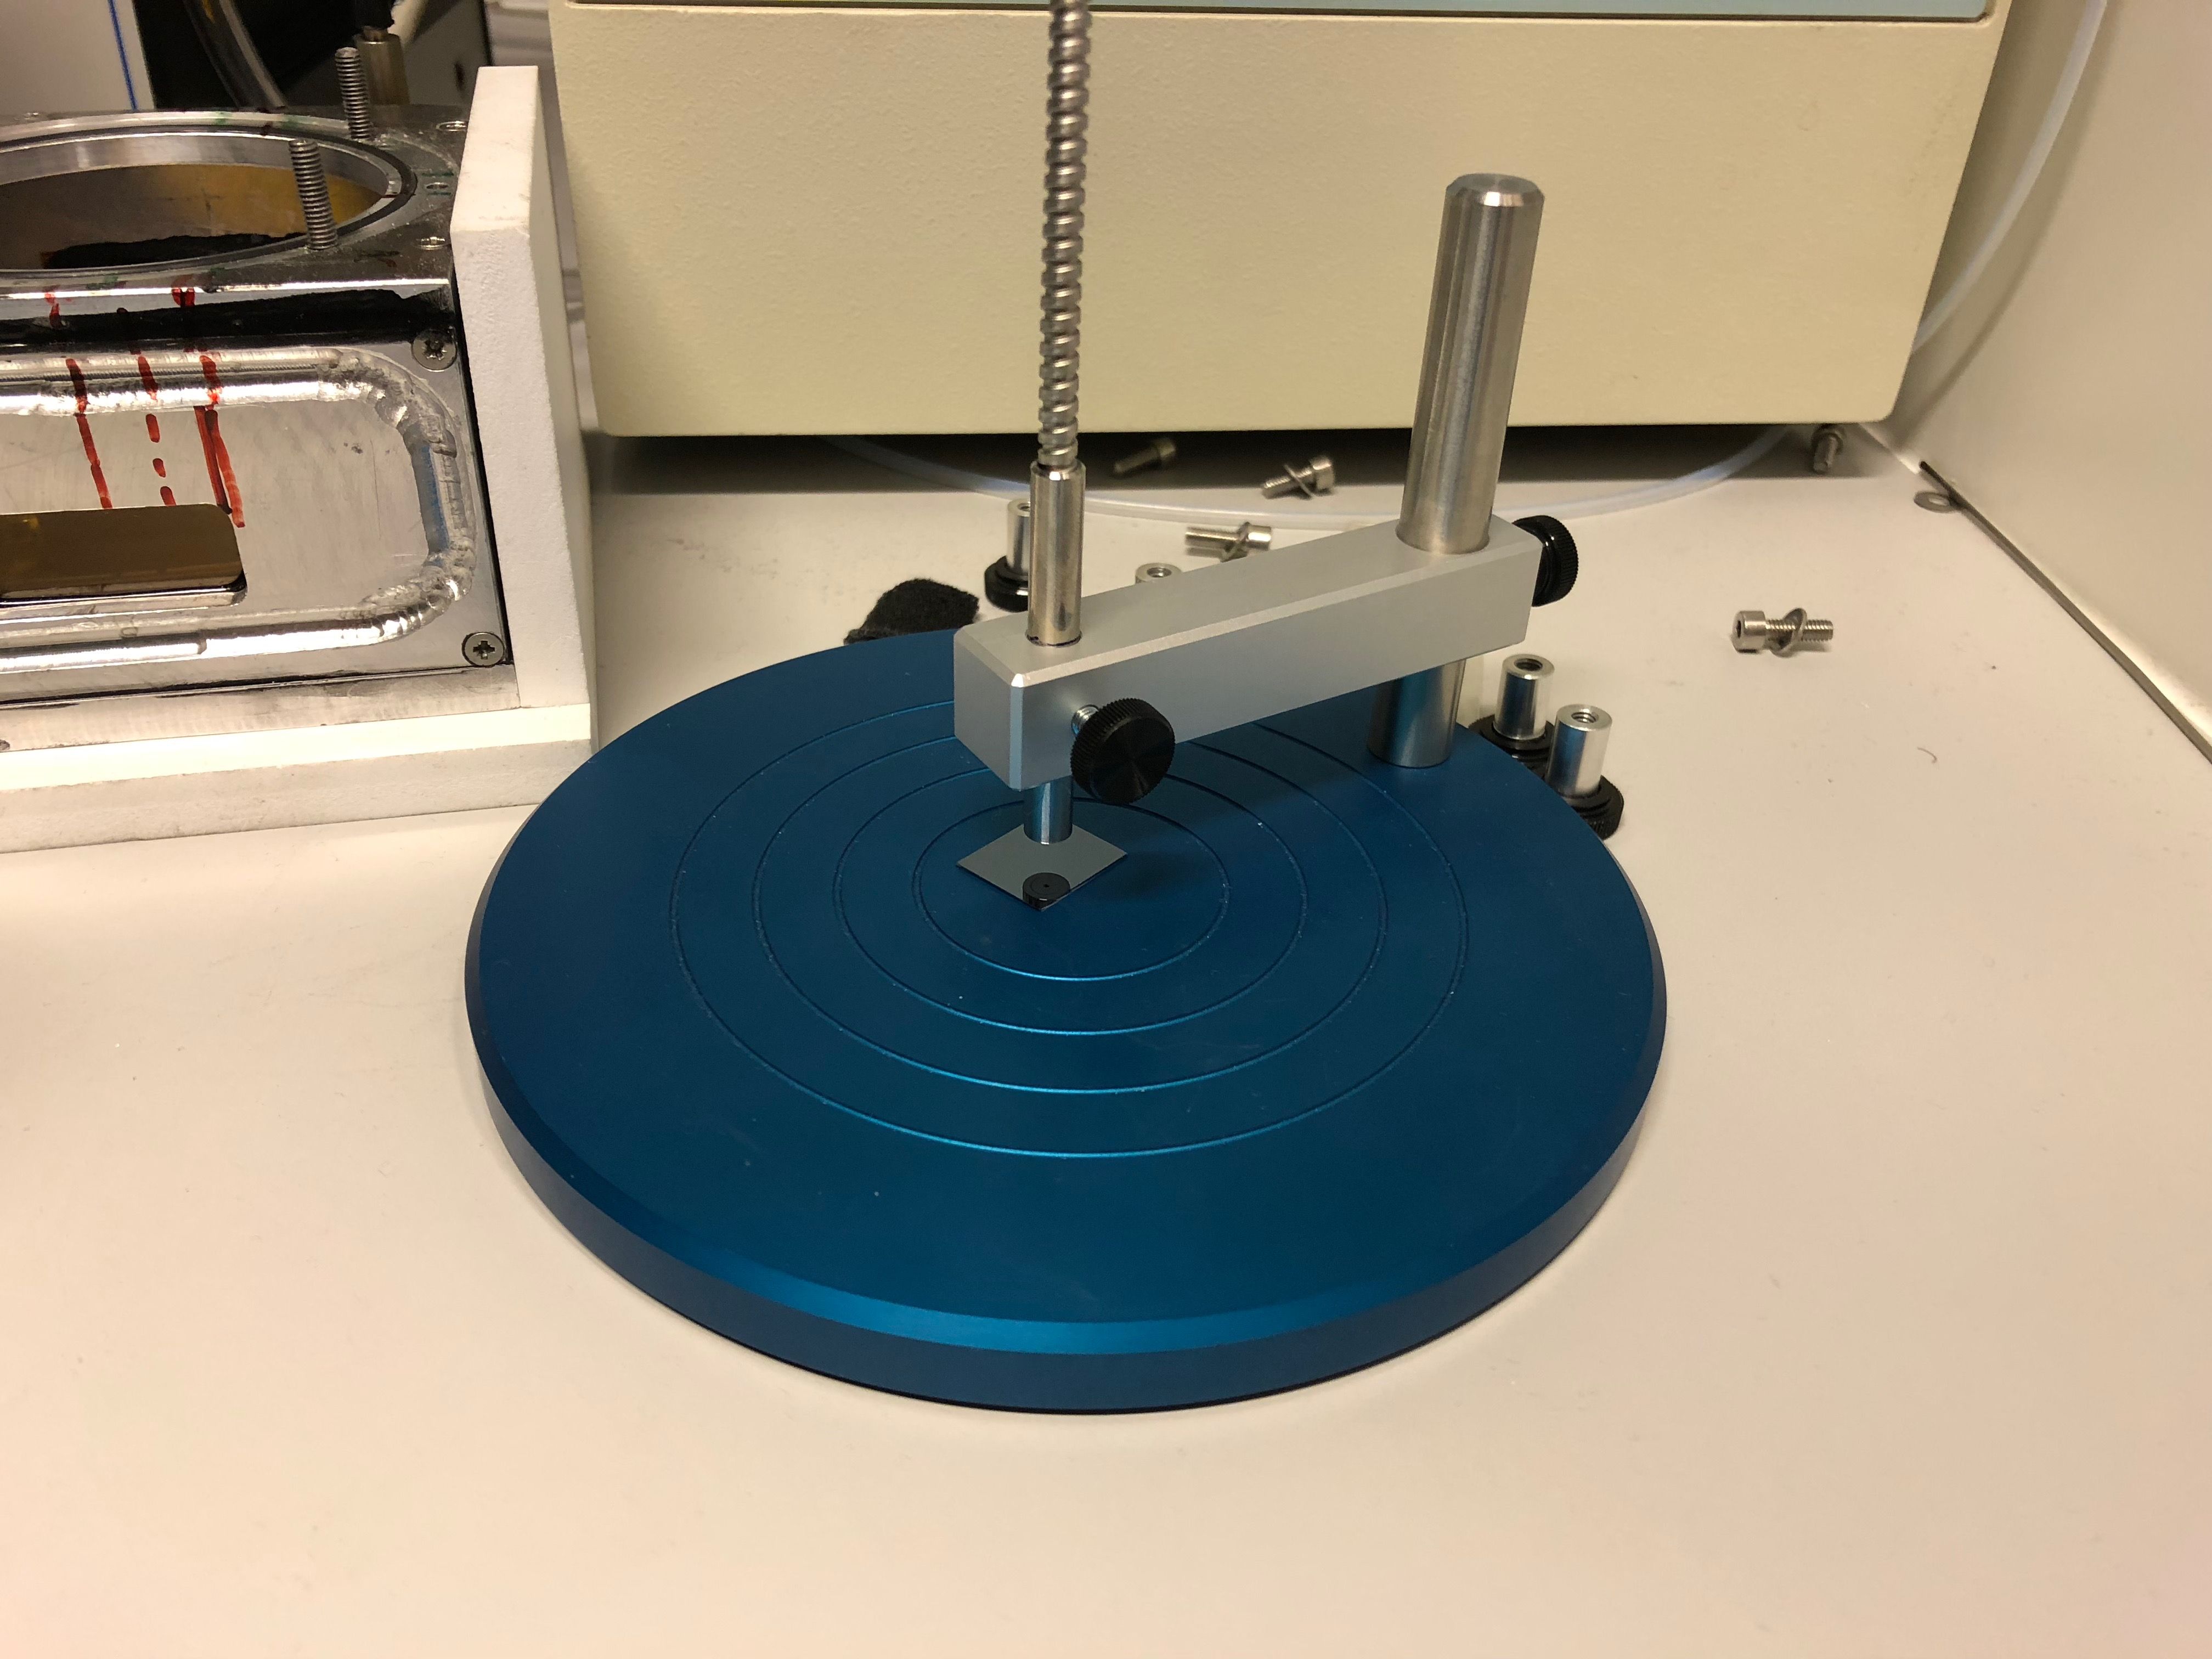
\includegraphics[scale=0.04]{setup3.JPG}
\end{figure}
\end{minipage}
\begin{minipage}{0.5\textwidth}
\begin{figure}
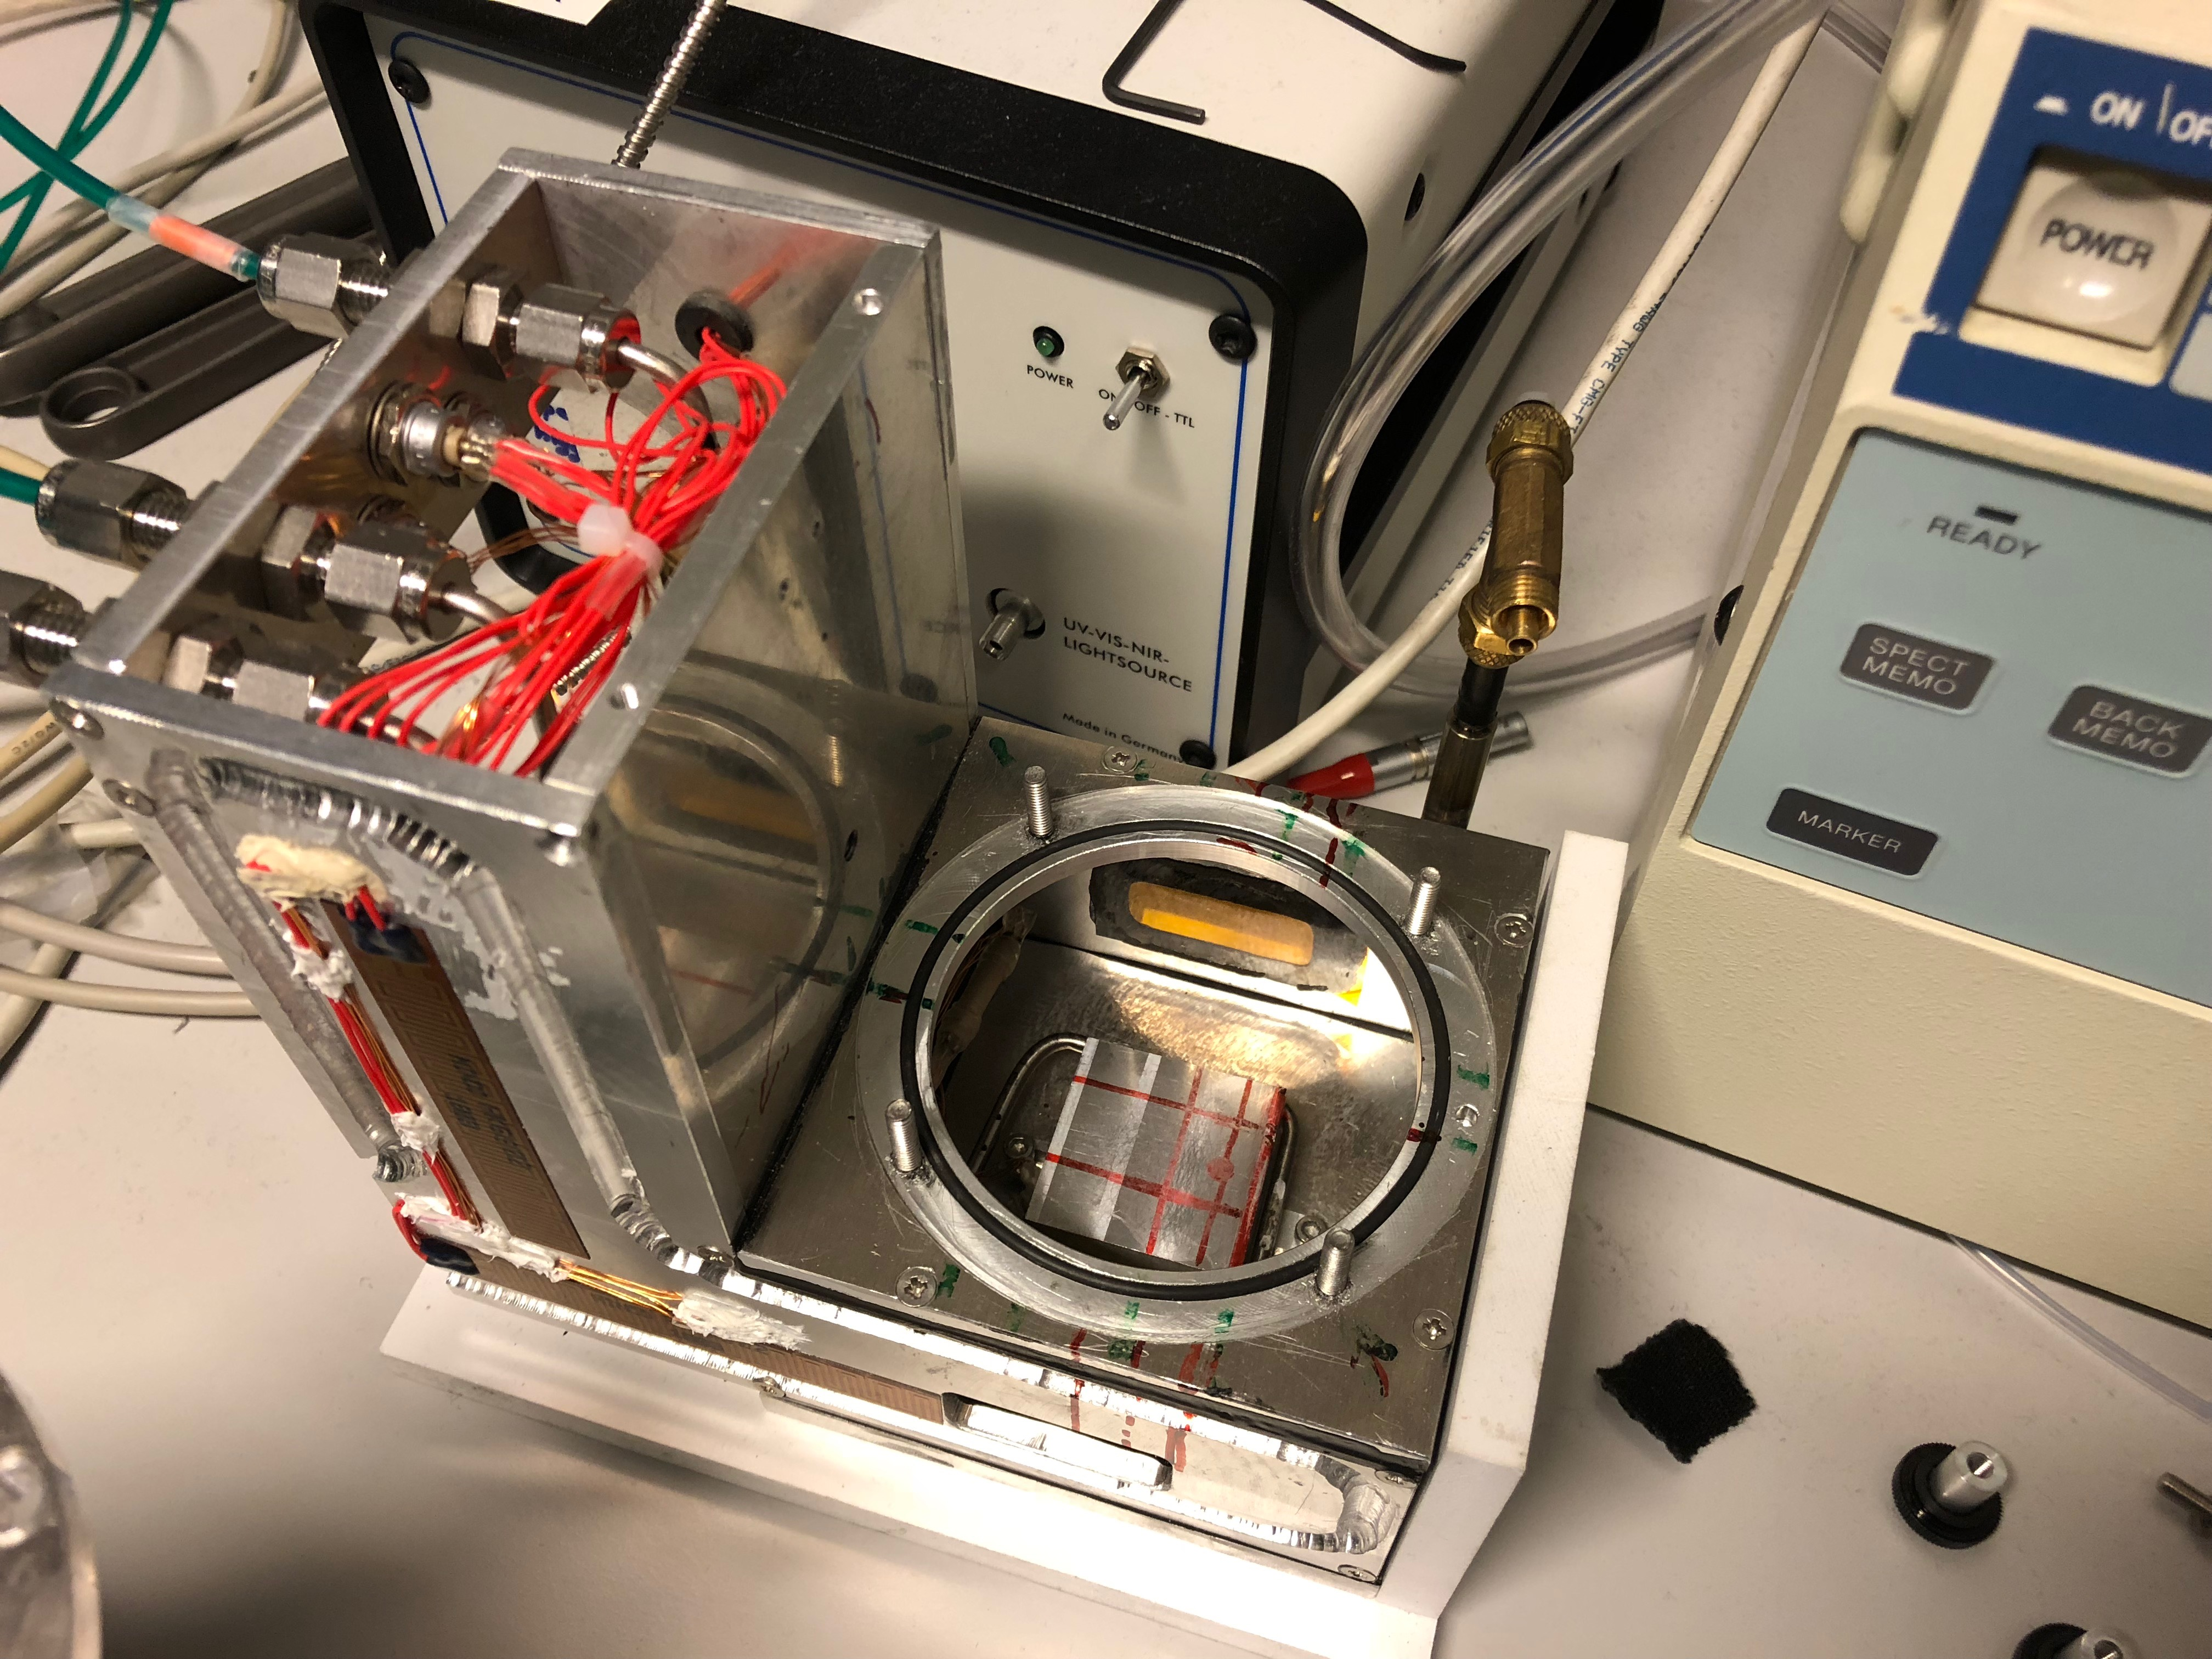
\includegraphics[scale=0.04]{setup4.JPG}
\end{figure}
\end{minipage}
\end{frame}

\begin{frame}{Step Wafer}
	\begin{figure}
	\centering
	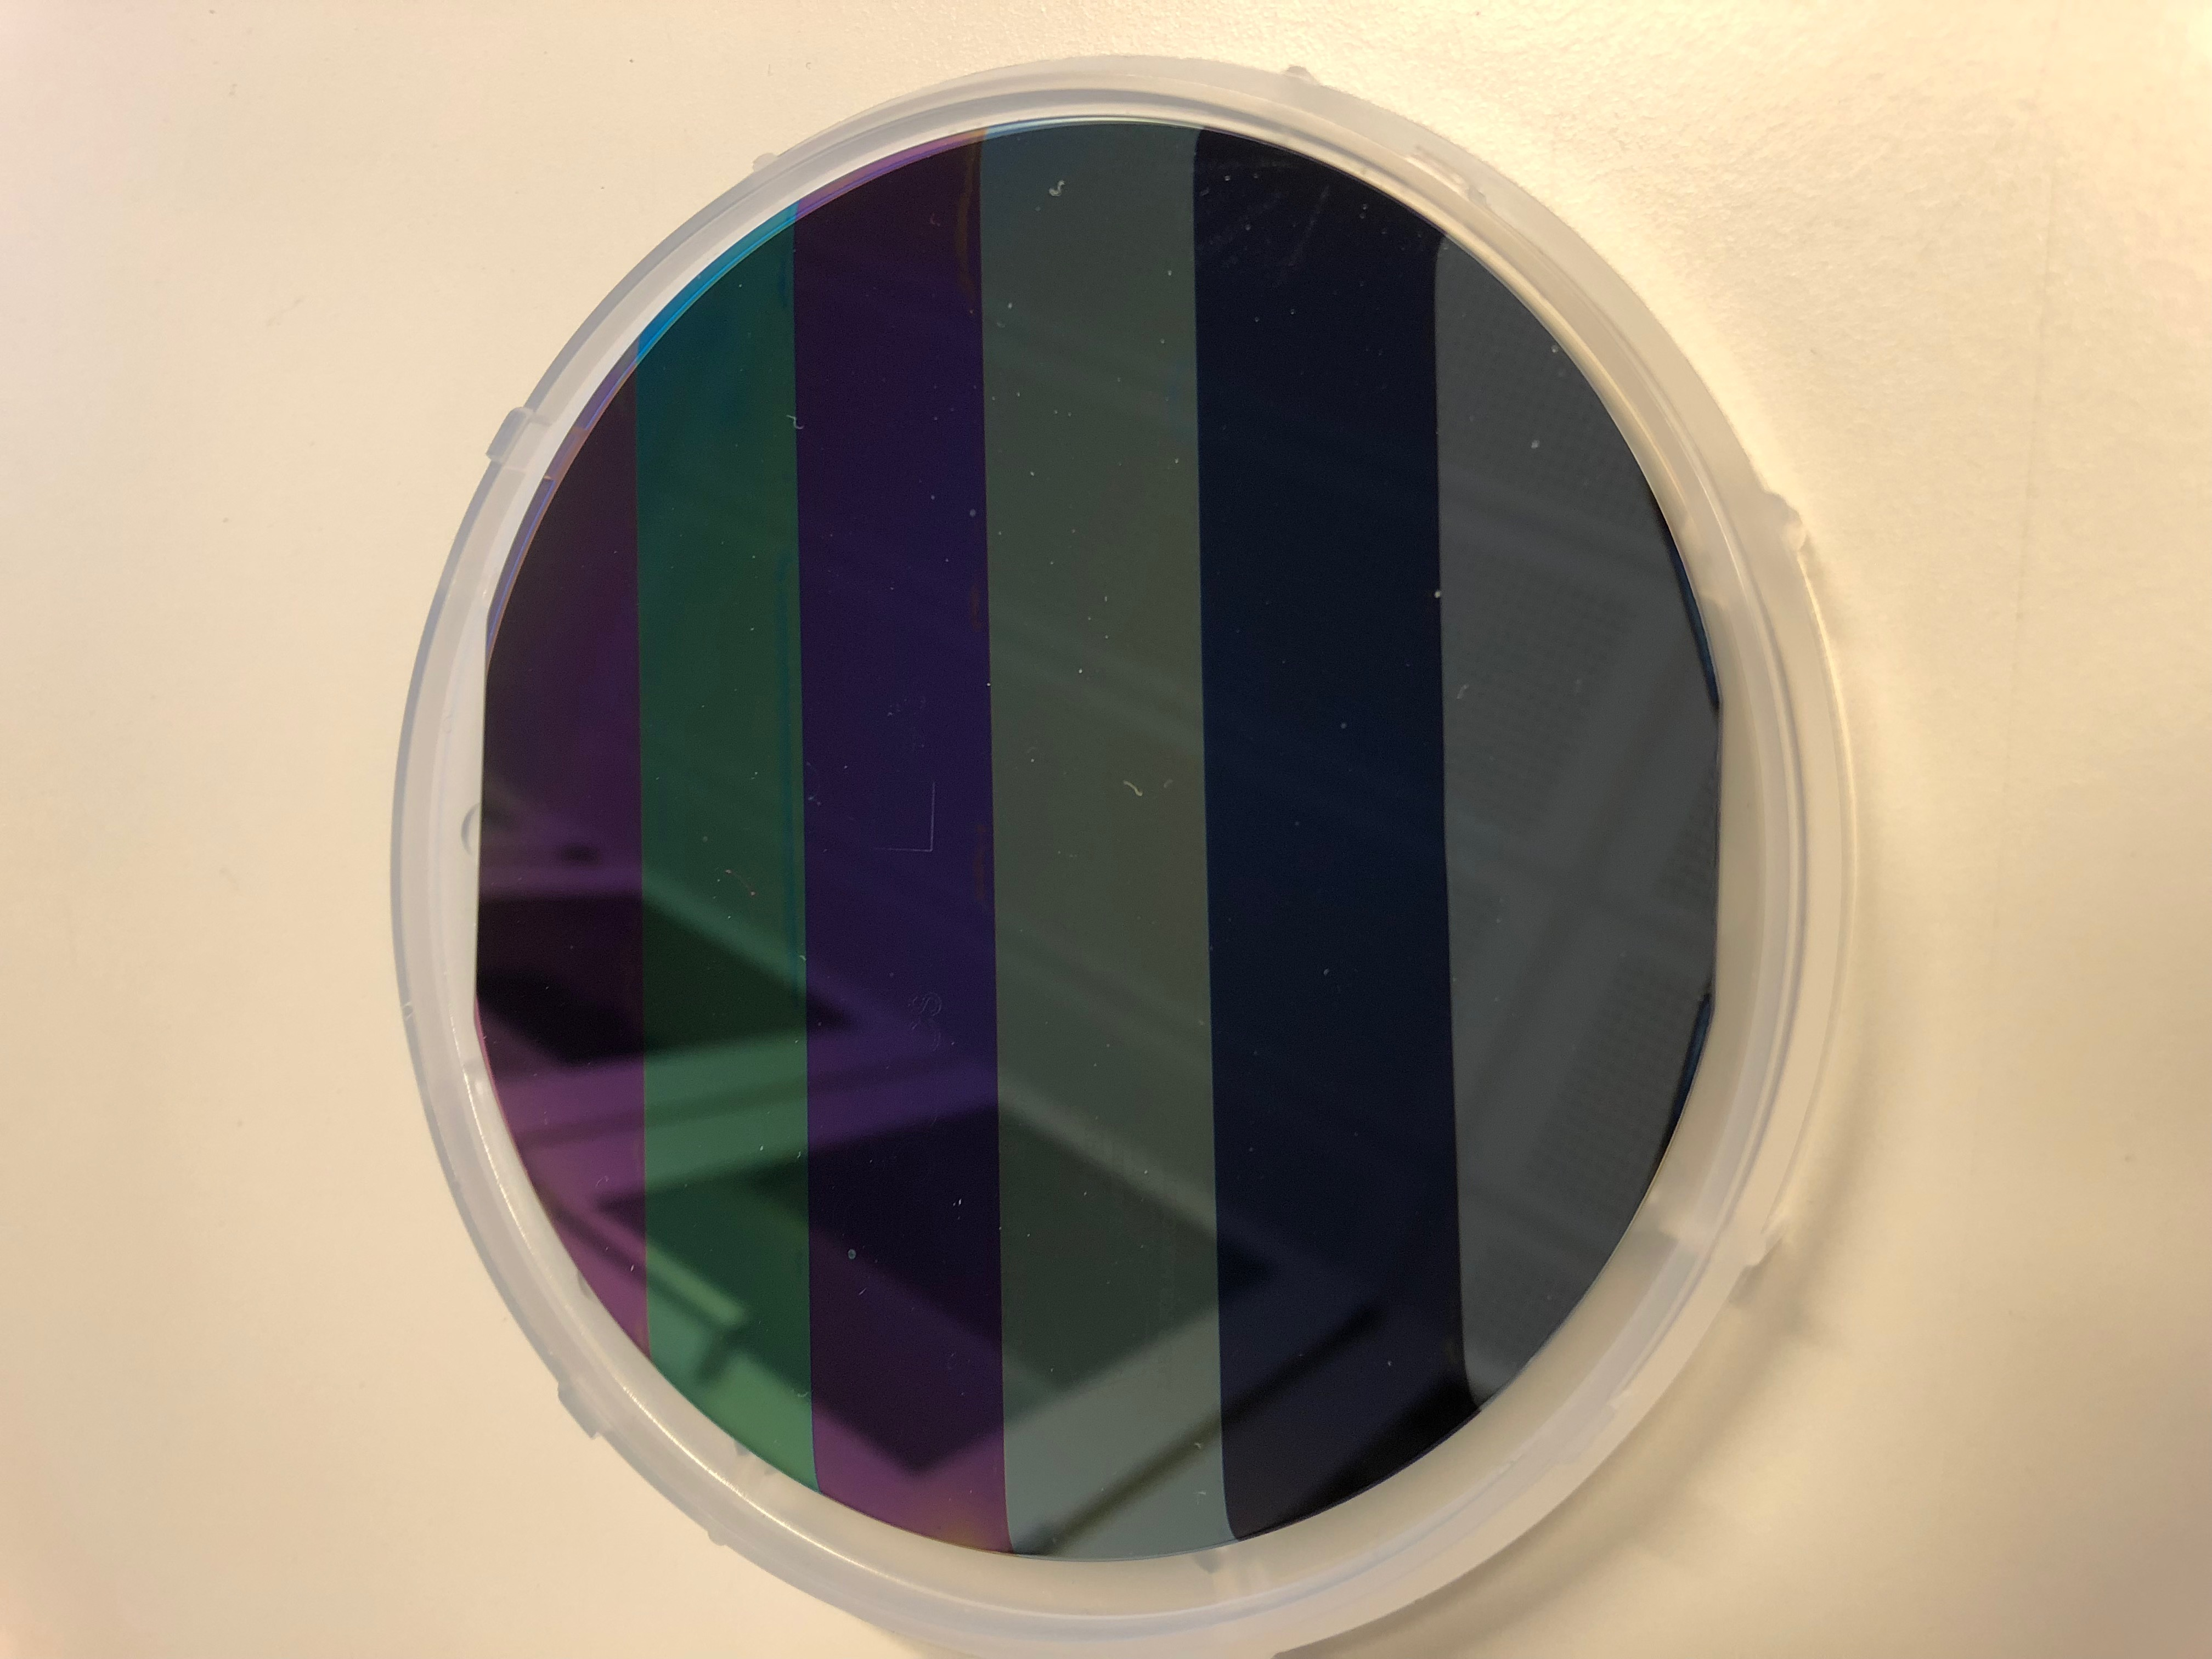
\includegraphics[scale=0.06,angle=-90]{stepwafer.JPG}
	\end{figure}
\end{frame}
	
	
\begin{frame}{NanoCalc Software}
	\begin{figure}
		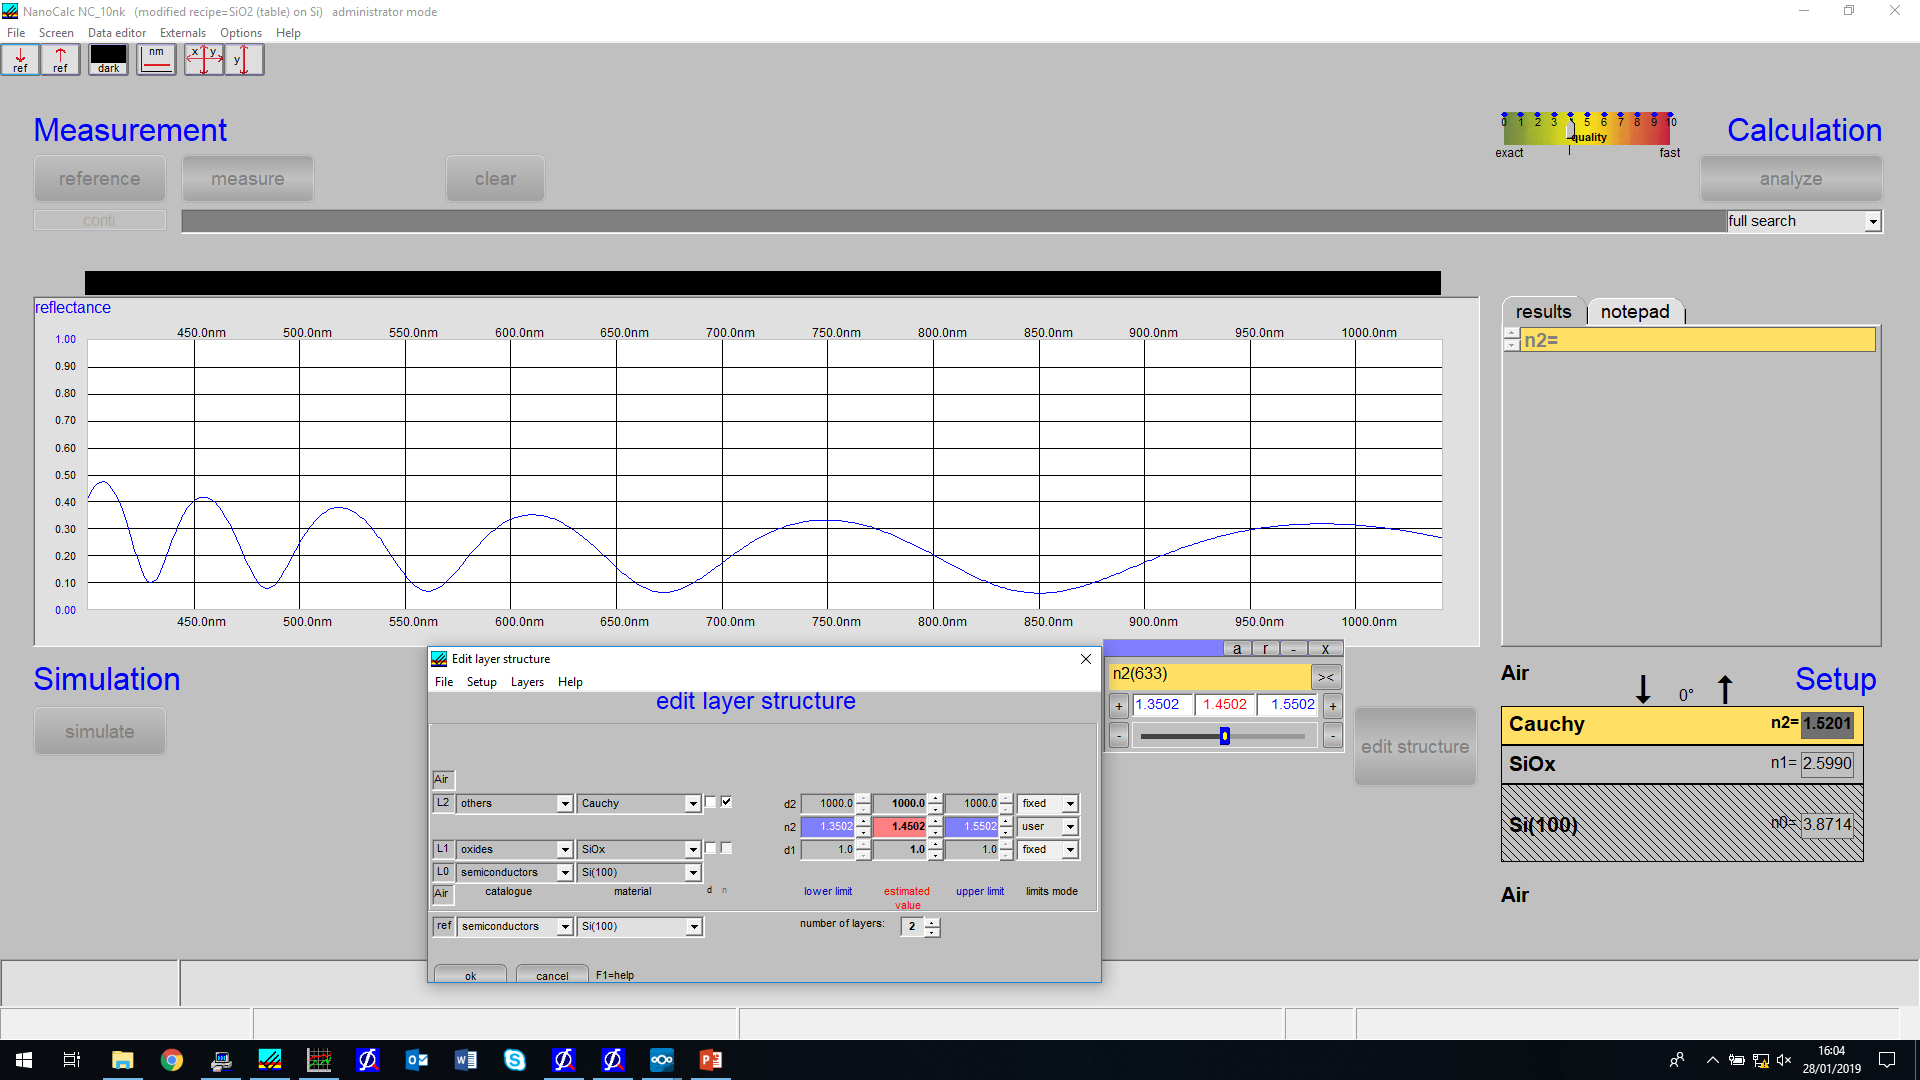
\includegraphics[width=\textwidth]{nanocalc.png}
	\end{figure}
\end{frame}

\begin{frame}{Taking Measurements}

\begin{equation*}
Reflectance = \frac{Meas-Dark}{Ref}\cdot R_{sub}
\end{equation*}

\begin{itemize}
\item Dark Measurement - $Dark$\\
\begin{itemize}
\item Measuring stray light.
\end{itemize}
\item Reference Measurement - $Ref$\\
\begin{itemize}
\item Measuring light from blank wafer - SiOx/Si
\item Ref data - minus dark
\end{itemize}
\item Wafer Measurement - $Meas$\\
\begin{itemize}
\item Wafer with spin-coated polymer
\end{itemize}
\item Reflectance from ambient/substrate model - $R_{sub}$
\begin{itemize}
\item Calculation - Fresnel model
\end{itemize}
\end{itemize}

\end{frame}



	\section{Polymers}
	
\begin{frame}{Polymers used in Master Thesis}    
    \begin{columns}[t]
        \column{.5\textwidth}
        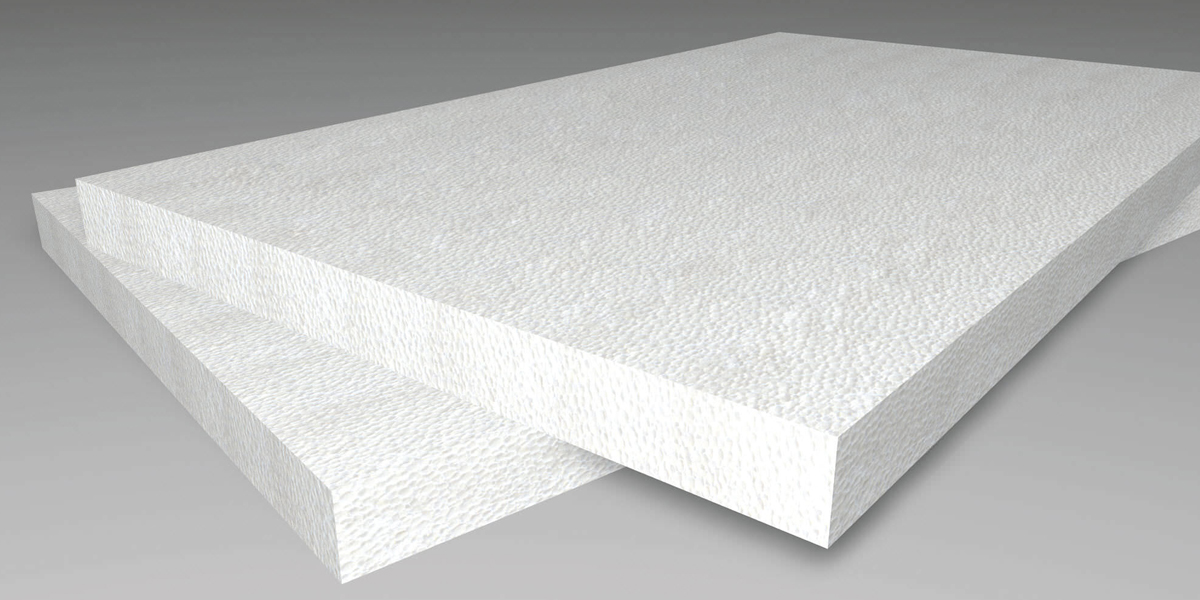
\includegraphics[width=\columnwidth,height=3cm]{pswebsite.jpg}
        \captionof{figure}{Source:www.isowall.co.za}
        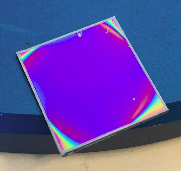
\includegraphics[width=\columnwidth,height=3cm]{PSphoto1.png}
        \captionof{figure}{Polystyrene wafer}
        \column{.5\textwidth}
        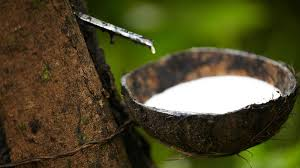
\includegraphics[width=\columnwidth,height=3cm]{piwebsite.jpeg}
        \captionof{figure}{Source:wbcsd.org}
        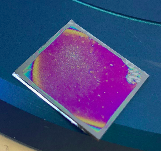
\includegraphics[width=\columnwidth,height=3cm]{PIphoto1.png}
        \captionof{figure}{Polyisoprene wafer}
    \end{columns}
\end{frame}

\begin{frame}{Polymers used in Master Thesis}
\centering
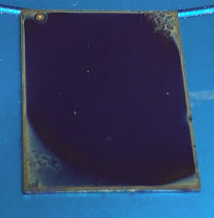
\includegraphics[scale=0.8]{PSbPIBsva.png}
\captionof{figure}{Polystyrene-b-polyisoprene}
\end{frame}

	

	
	\section{Fresnel Models}
	
\begin{frame}{Fresnel Equations - Substrate}

		\begin{figure}
			\hfill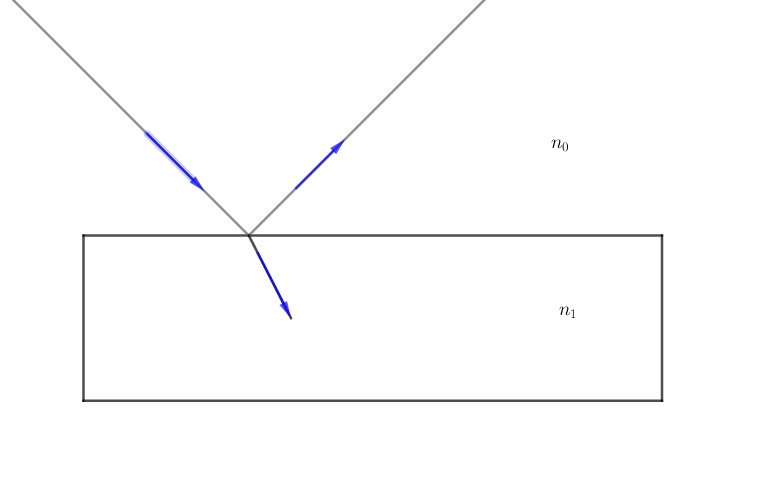
\includegraphics[width = \textwidth]{subrefl.png}\hspace*{\fill}
		\end{figure}
		\begin{equation*}
			r_p = \frac{E_{r,p}}{E_{i,p}} = \frac{N_1-N_0}{N_0+N_1}
		\end{equation*}
		\begin{equation*}
			R_p = \mid r_p \mid ^2 
		\end{equation*}

	
%	\begin{minipage}{0.6\textwidth}
%		\begin{figure}
%		\centering
%		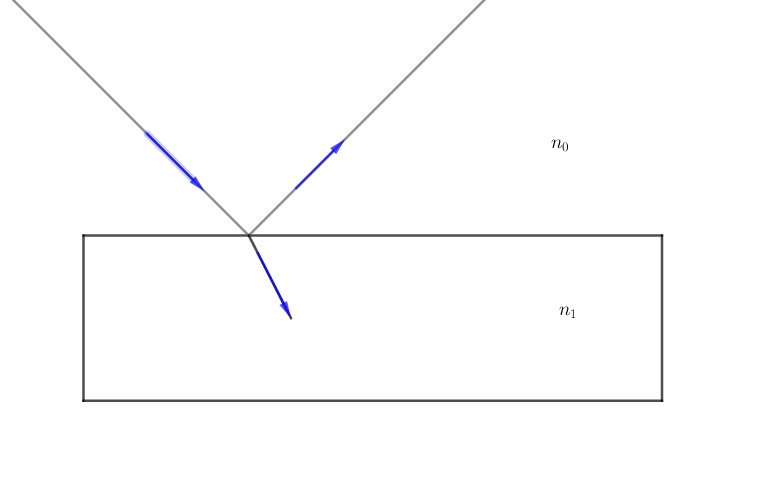
\includegraphics[scale=0.3]{subrefl.png}
%		\end{figure}
%	\end{minipage}
%	\begin{minipage}{0.4\textwidth}
%		\begin{equation*}
%			r_p = \frac{E_{r,p}}{E_{i,p}} = \frac{n_1-n_0}{n_0+n_1}
%		\end{equation*}
%		\begin{equation*}
%			R_p = \mid r_p \mid ^2 
%		\end{equation*}
%	\end{minipage}

\end{frame}
	
\begin{frame}{Fresnel Equations - One layer}
	
	\begin{figure} 
		 \begin{center}
		   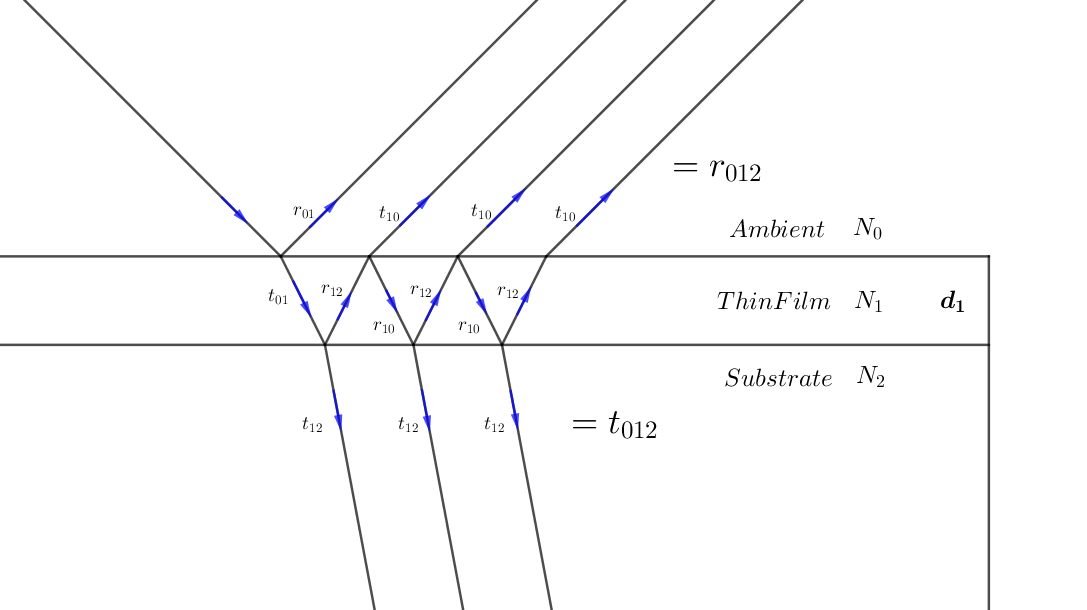
\includegraphics[width=\textwidth]{figrefl.png}
		 \end{center}
	\end{figure}
	\begin{align*}
	r_{012} = &r_{01} + t_{01}t_{10}r_{12}\exp(-i2\beta) + t_{01}t_{10}r_{10}r_{12}^2\exp(-i4\beta)+ \\ &t_{01}t_{10}r_{10}^2r_{12}^3\exp(-i6\beta)+ \cdots
	\end{align*} 
	
\end{frame}
	
\begin{frame}{Fresnel Equations - One layer}
	
	\begin{align*}
	r_{012} &= \frac{r_{01}+r_{12}\exp(-i2\beta)}{1+r_{01}r_{12}\exp(-i2\beta)}\\
	r_{jk} &= \frac{N_k-N_j}{N_j+N_k}\\
	\beta &=\frac{2\pi d_1}{\lambda} N_1\\
	R_{012} &= \mid r_{012} \mid ^2 
	\end{align*}	
	
\end{frame}

\begin{frame}{Homopolymer Fresnel Model}
	\begin{figure}
	\centering
	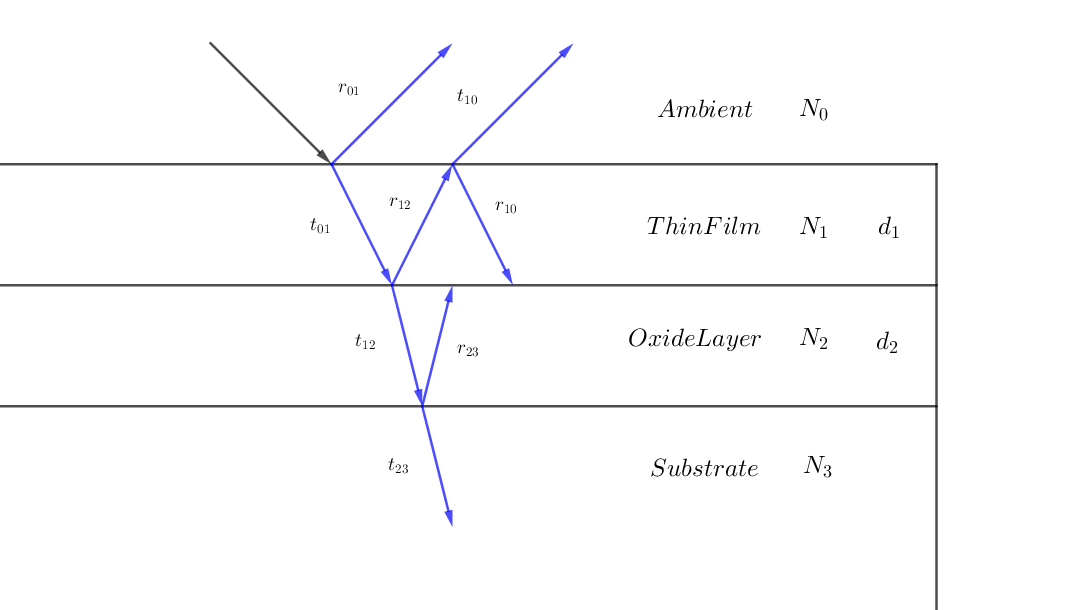
\includegraphics[width=\textwidth]{figmulti1.png}
	\end{figure}
\end{frame}
\begin{frame}{Homopolymer Fresnel equations}


\begin{align*}
r_{0123} &= \frac{r_{01}+r_{123}\exp{(-i2\beta_1)}}{1+r_{01}r_{123}\exp{(-i2\beta_1)}}\\
r_{123} &= \frac{r_{12}+r_{23}\exp{(-i2\beta_2)}}{1+r_{12}r_{23}\exp{(-i2\beta_2)}}\\
r_jk &= \frac{N_k-N_j}{N_j+N_k}\\
R_{0123} &= \mid r_{0123} \mid ^2 \\
\beta_i &= \frac{2\pi d_i}{\lambda}N_i
\end{align*}

$N_0$,$N_1$ and $d_1$ fitted during solvent vapour annealing.

\end{frame}

\begin{frame}{Diblock copolymer Fresnel model}
	\begin{figure}
	\centering
	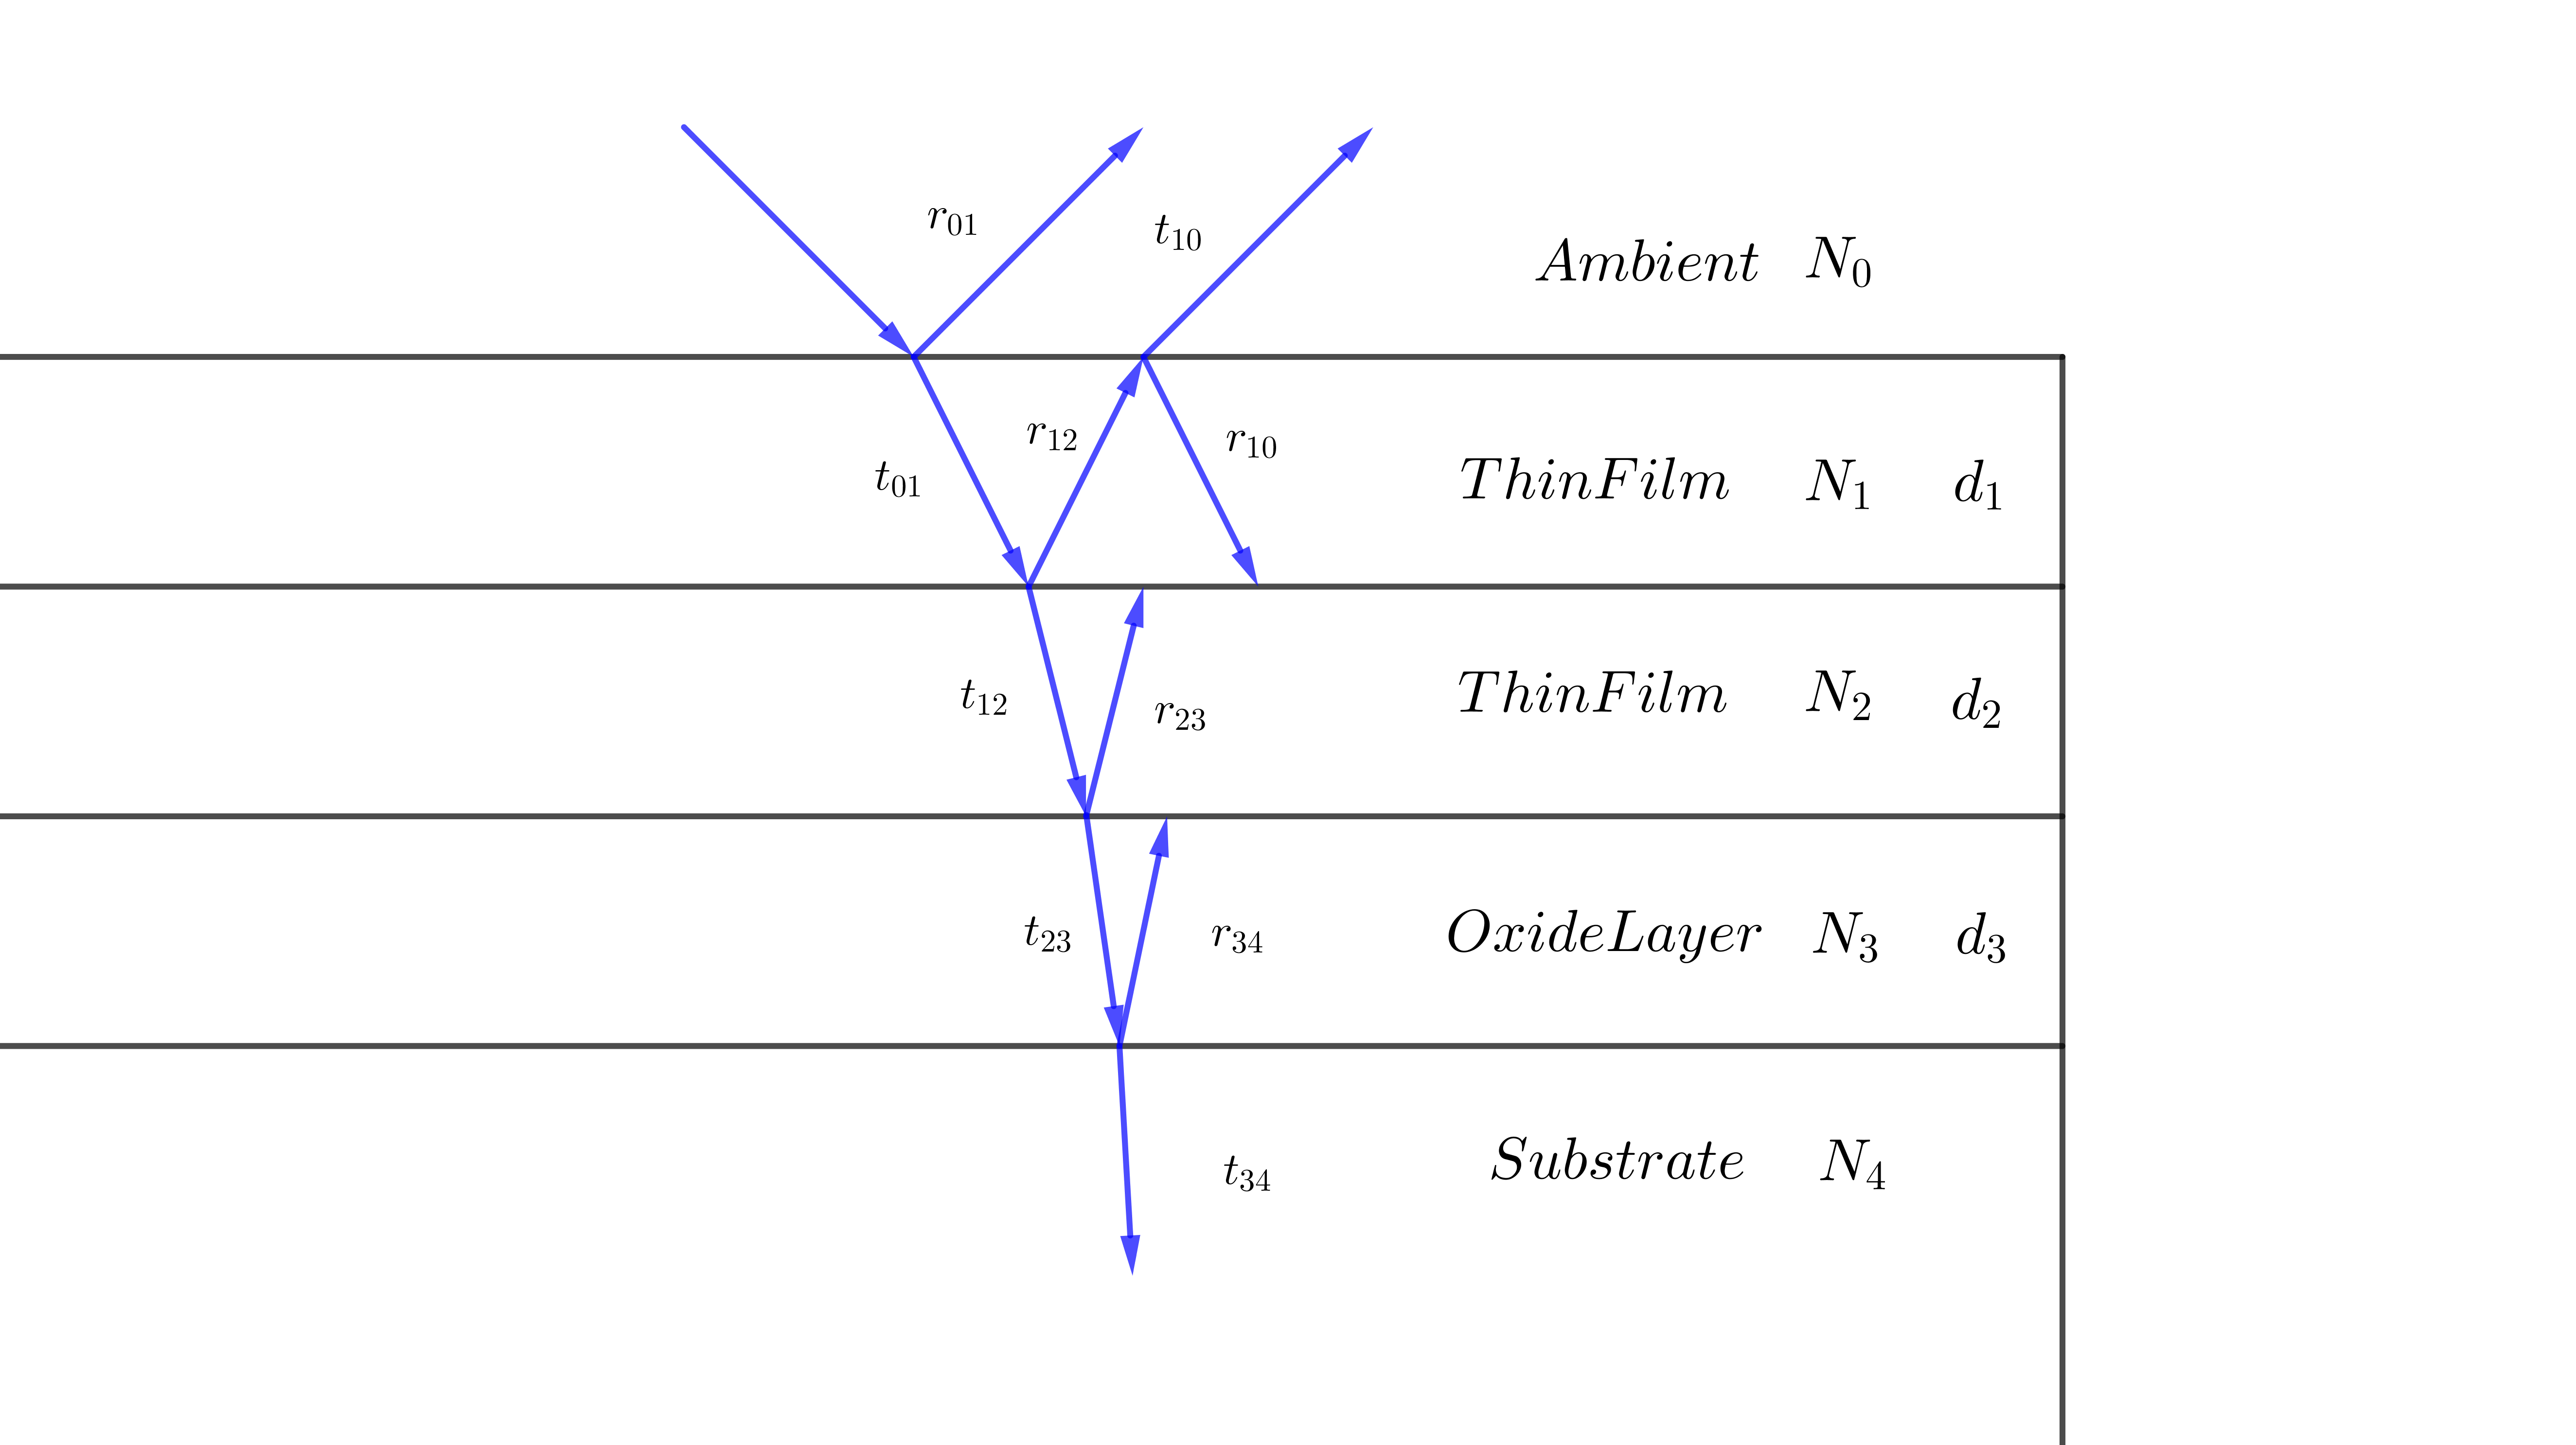
\includegraphics[width=\textwidth]{diblock.png}
\end{figure}
\end{frame}

\begin{frame}{Diblock copolymer Fresnel Equations}

\begin{align*}
r_{01234}&= \frac{r_{01}+r_{1234}\exp(-i2\beta_1)}{1+r_{01}r_{1234}\exp(-i2\beta_1)} \\
r_{1234} &= \frac{r_{12}+r_{234}\exp(-i2\beta_2)}{1+r_{12}r_{234}\exp(-i2\beta_2)} \\
r_{234}  &= \frac{r_{23}+r_{34}\exp(-i2\beta_3)}{1+r_{23}r_{34}\exp(-i2\beta_3)} \\
r_{jk}   &= \frac{N_k-N_j}{N_k + N_j}\\  
\beta_i  &= \frac{2\pi d_i}{\lambda}N_i
\end{align*}

$N_0$,$N_1$,$N_2$,$d_1$ and $d_2$ fitted during solvent vapour annealing.
\end{frame}

\begin{frame}{Plotted Fresnel models}
\begin{center}
\Huge Movie:varyRI.avi
\end{center}
\end{frame}	

	\section{Solvent vapour Annealing}
\begin{frame}{SVA protocol}
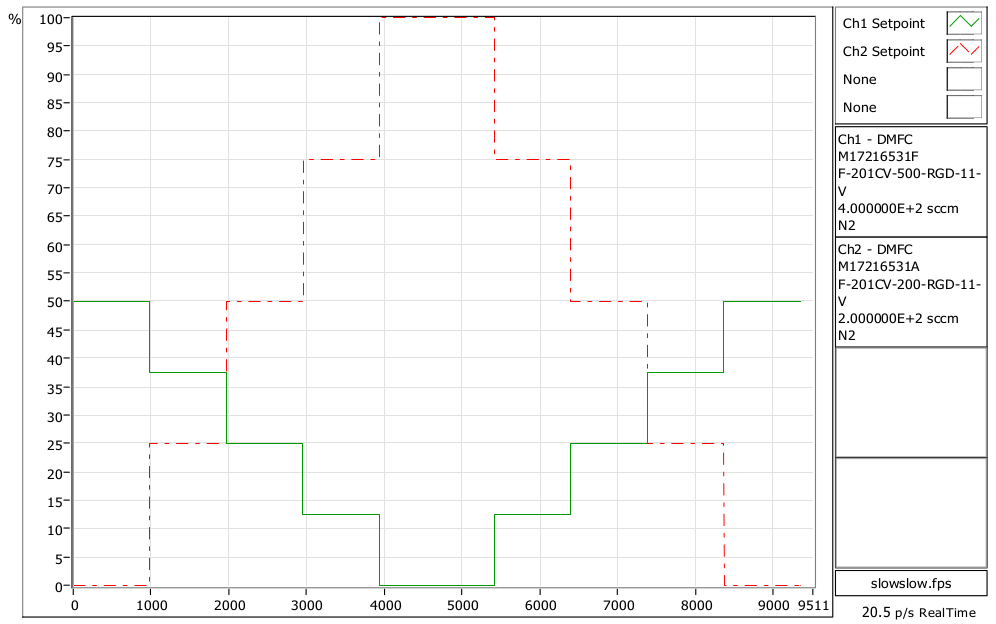
\includegraphics[width=\textwidth]{slowslowprotocol.png}
\end{frame}


	\section{Preliminary Studies}
	
\begin{frame}{Light Fluctuation}
\centering
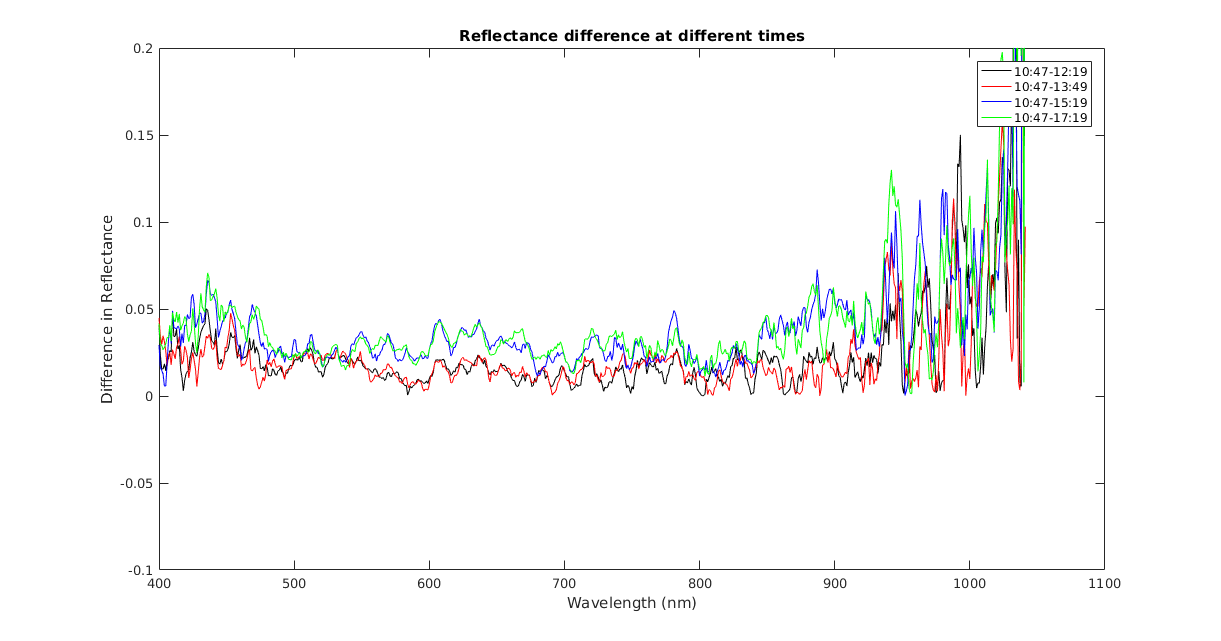
\includegraphics[width=\textwidth]{lightfluct1abs.png}
\captionof{figure}{Light Fluction study 1}
\end{frame}
\begin{frame}{Light Fluctuation continued}
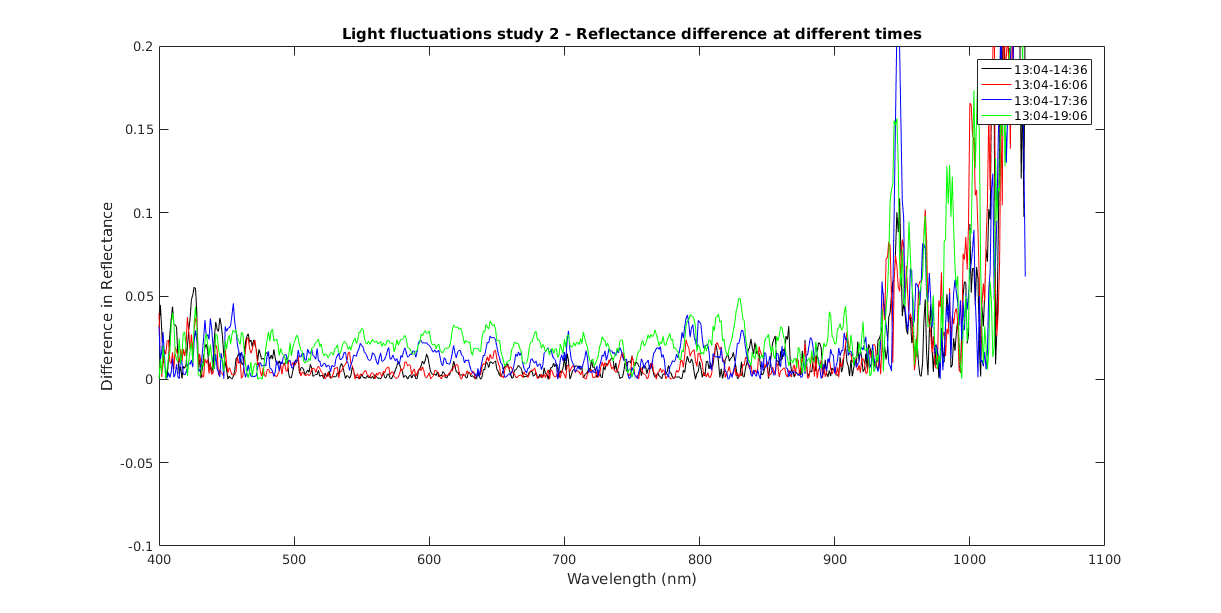
\includegraphics[width=\textwidth]{lightfluct2abs.png}
\captionof{figure}{Light Fluction study 2}
\end{frame}

\begin{frame}{Solvent vapour annealing ambient study}
\centering
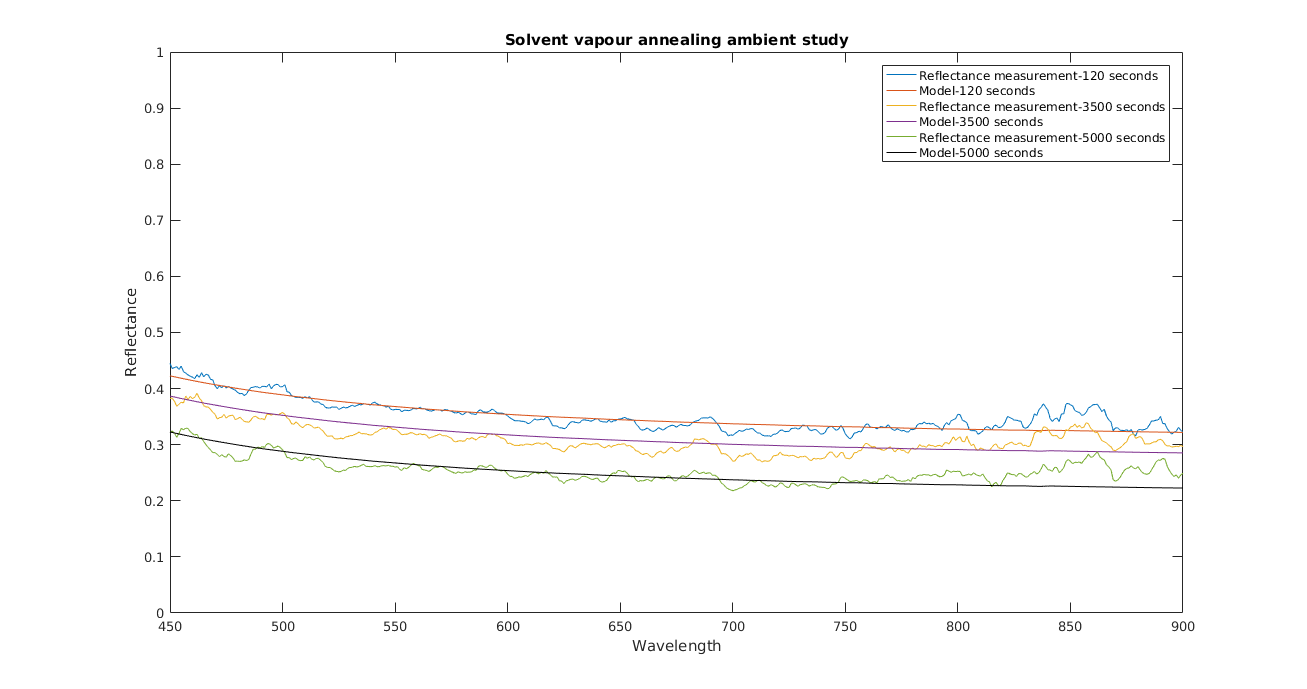
\includegraphics[height=0.35\textheight]{ambientreflectancestep.png}
\captionof{figure}{Reflectance curves at different times during SVA -120s,3500s,5000s.}
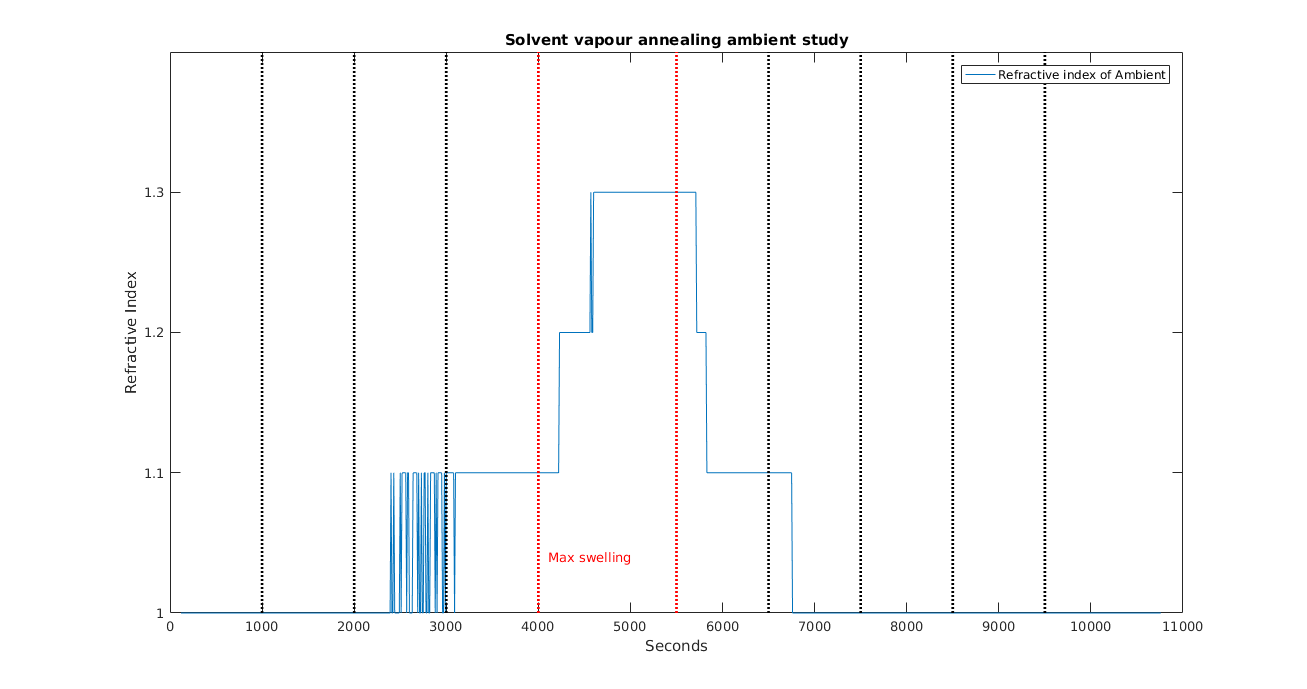
\includegraphics[height=0.35\textheight]{ambientstudyrefr.png}
\captionof{figure}{Ambient refractive index}
\end{frame}


	\section{Results - 1 polymer layer}

\begin{frame}{Polystyrene}
\begin{center}
\Huge Movie: PSsva.avi
\end{center}
\end{frame}

\begin{frame}{Polystyrene Results}
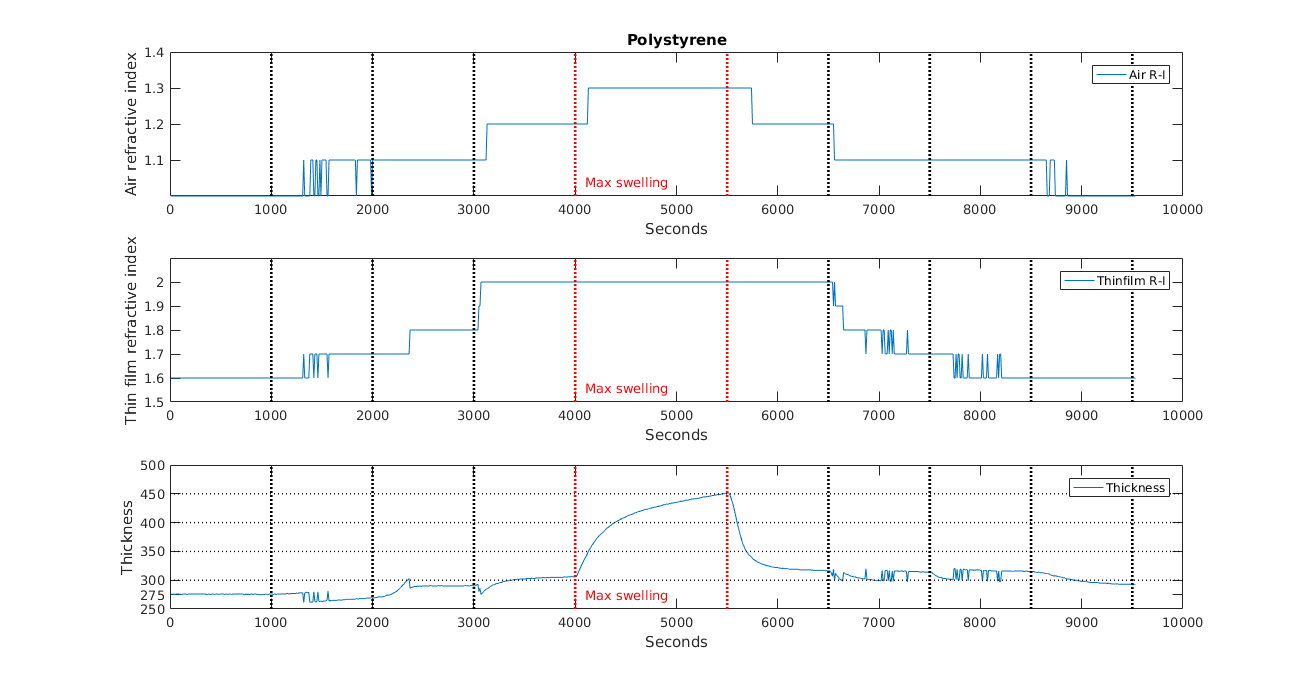
\includegraphics[width=\textwidth]{PSswelling1.png}
\end{frame}

\begin{frame}{Polystyrene MSE}
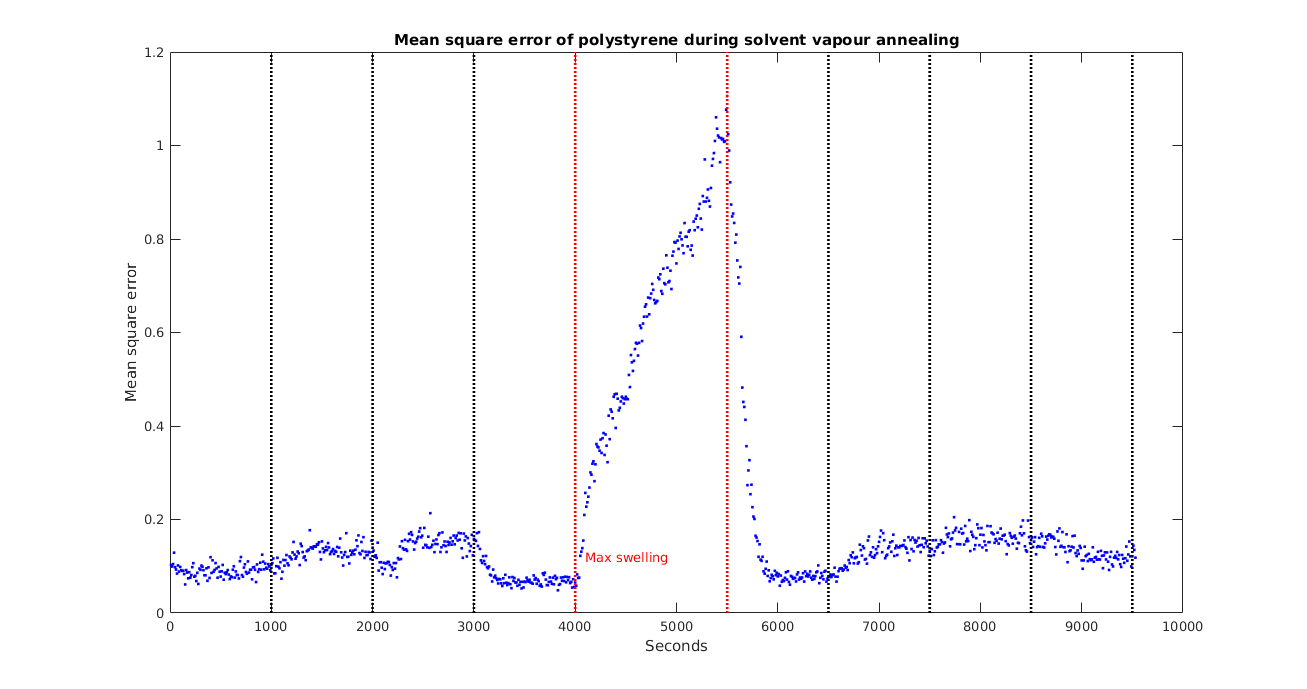
\includegraphics[width=\textwidth]{PSswelling2.png}
\end{frame}


\begin{frame}{Polystyrene comparison}
	\centering
	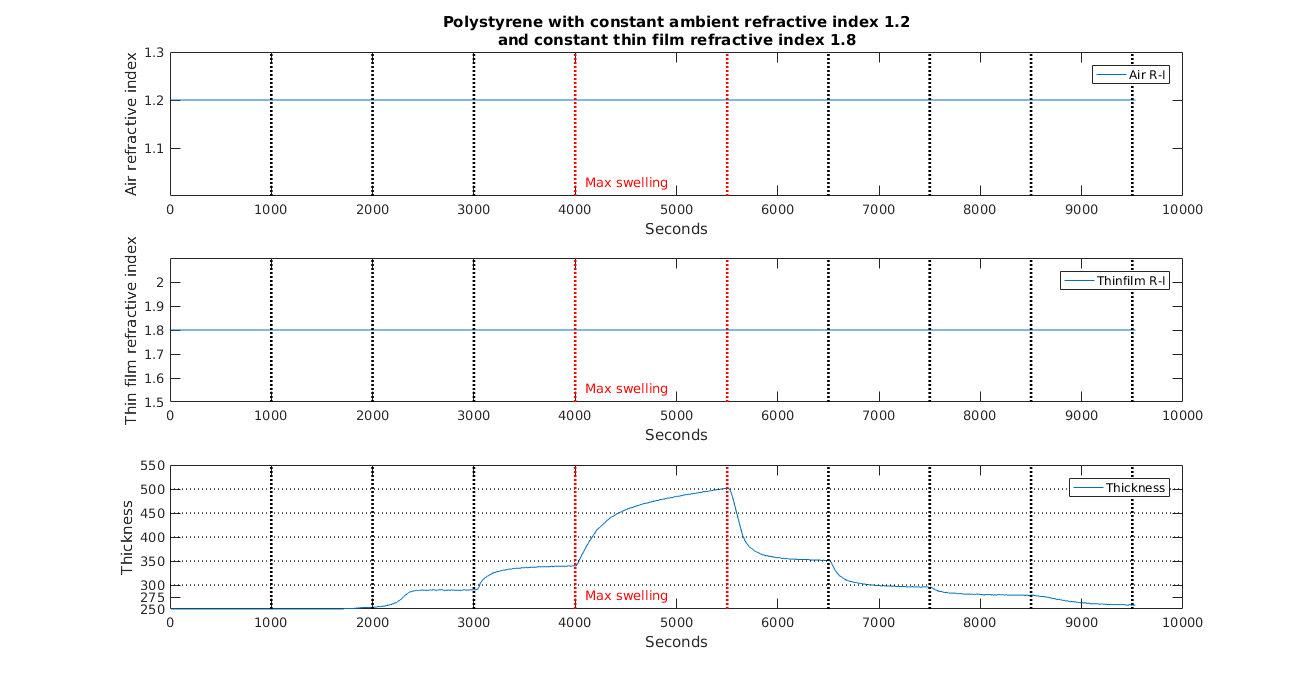
\includegraphics[width=\textwidth]{PSn12n18AVG1.png}
\end{frame}

\begin{frame}{Polystyrene comparison}
	\centering
	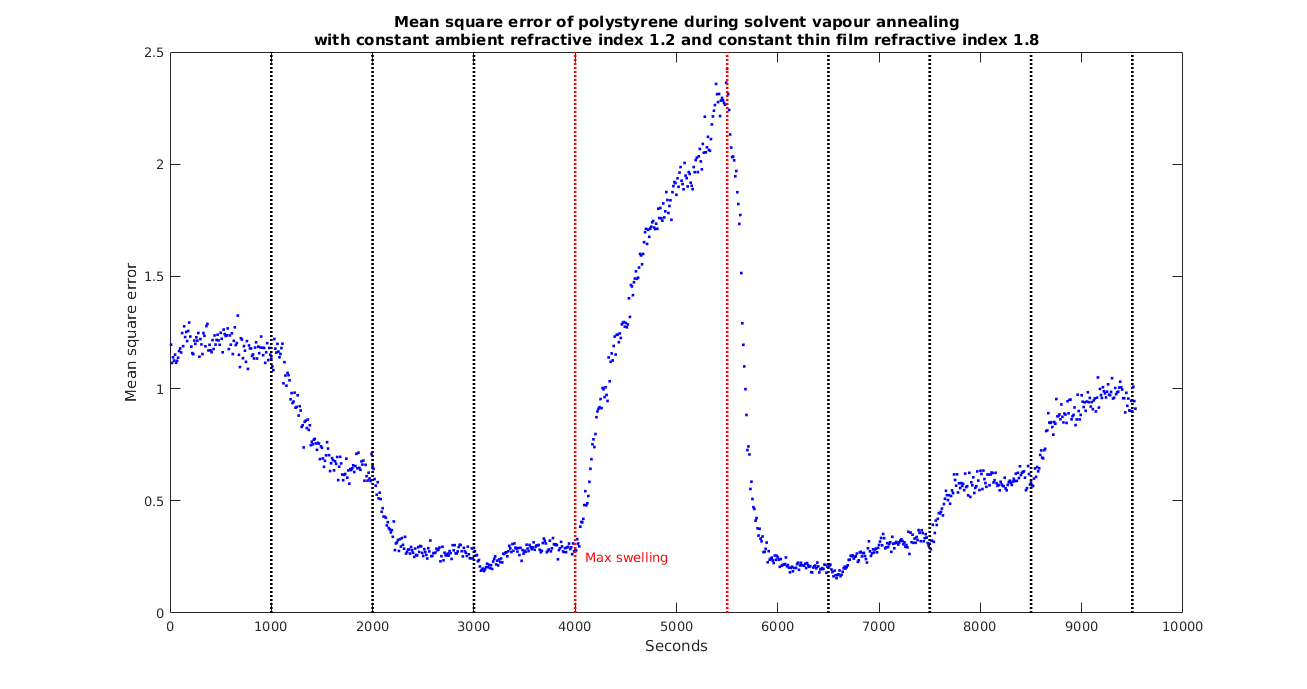
\includegraphics[width=\textwidth]{PSn12n18AVG2.png}\
\end{frame}


\begin{frame}{Polyisoprene}
\begin{center}
\Huge Movie:PIsvaframevalue2.avi
\end{center}
\end{frame}

\begin{frame}{Polyisoprene Results}
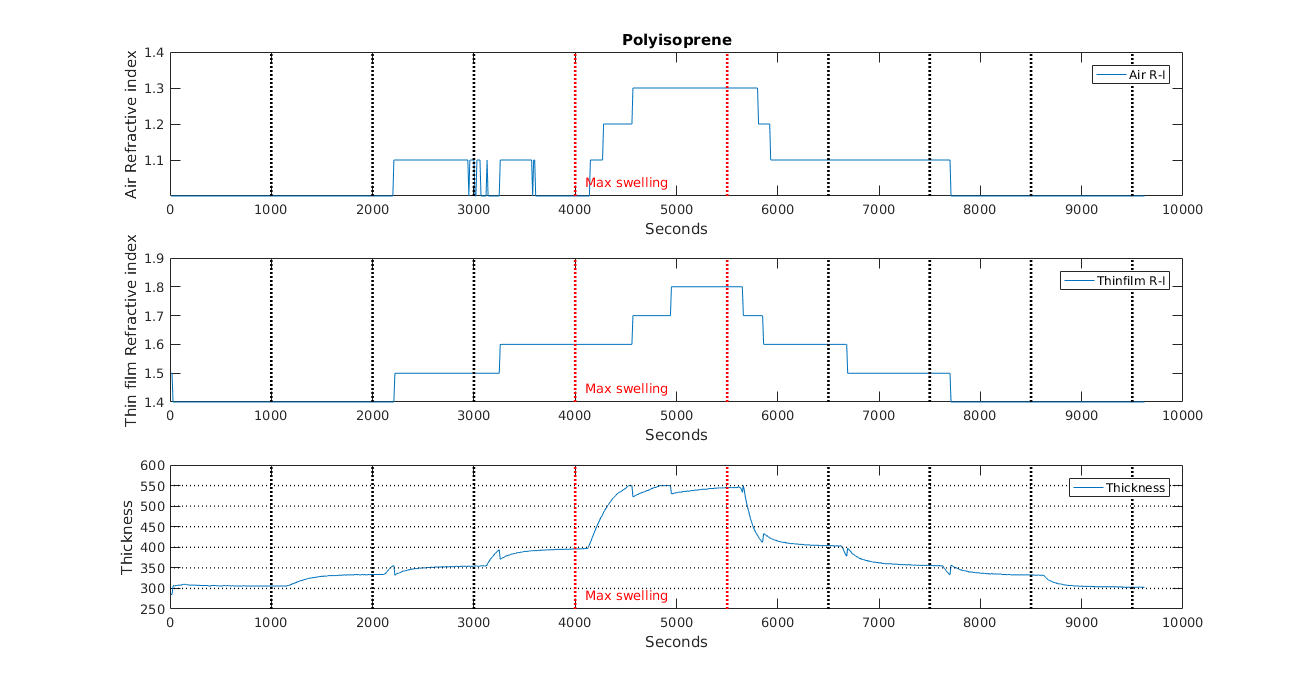
\includegraphics[width=\textwidth]{PIswelling1.png}
\end{frame}

\begin{frame}{Polyisoprene MSE}
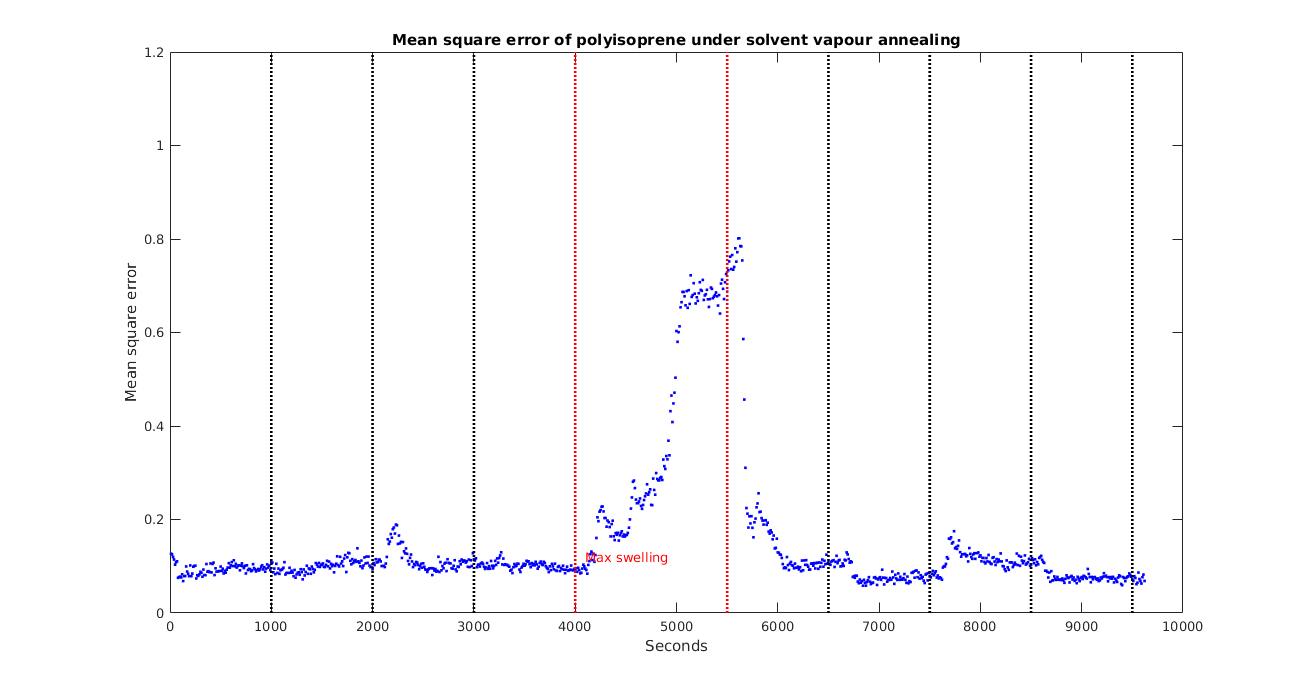
\includegraphics[width=\textwidth]{PIswelling2.png}
\end{frame}

\begin{frame}{Polyisoprene comparison}
	\centering
	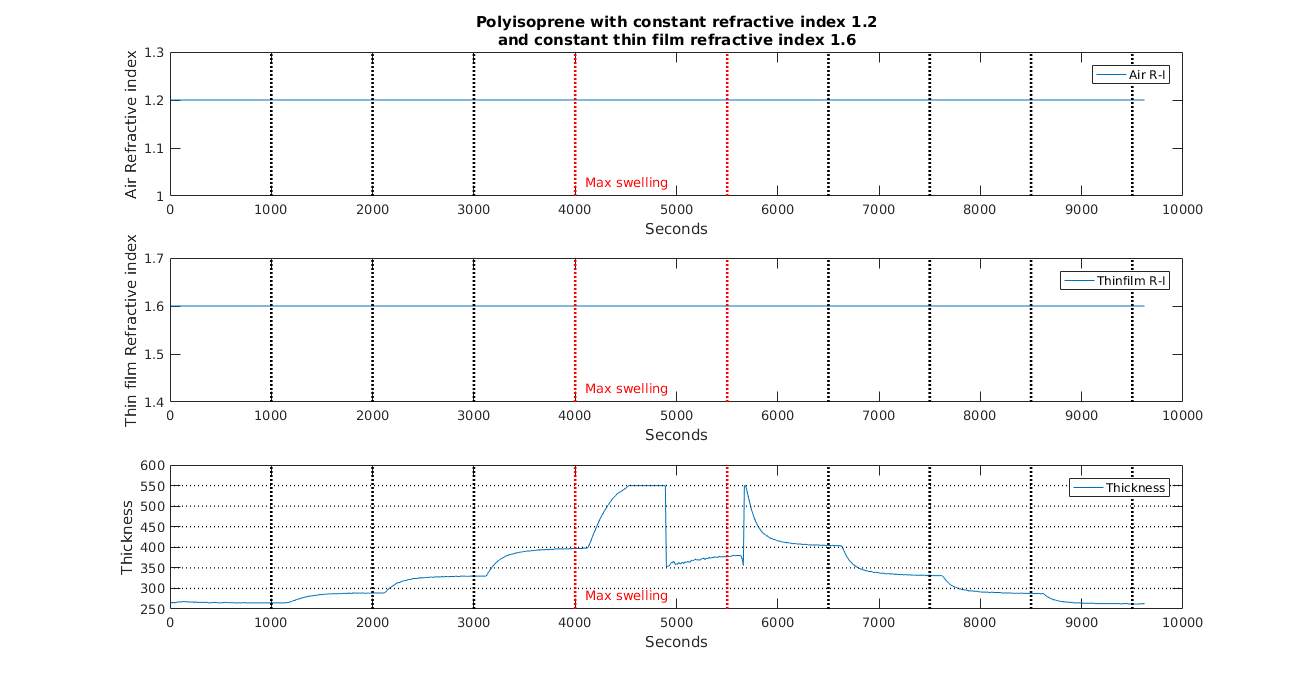
\includegraphics[width=\textwidth]{PIn12n16AVG1.png}
\end{frame}

\begin{frame}{Polyisoprene comparison}
	\centering
	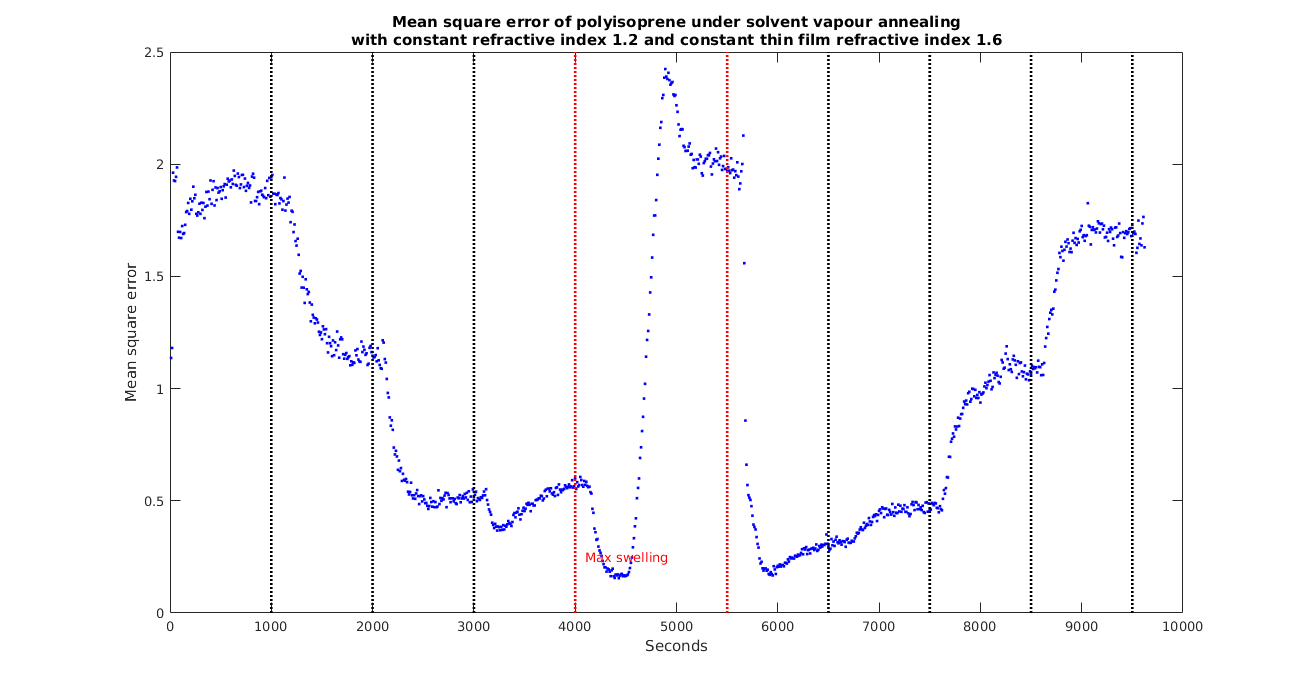
\includegraphics[width=\textwidth]{PIn12n16AVG2.png}\
\end{frame}

\begin{frame}{Polystyrene-b-polyisoprene}
\begin{center}
\huge Movie: PSbPIsinglemodel.avi
\end{center}
\end{frame}

\begin{frame}{Polystyrene-b-polyisoprene Results}
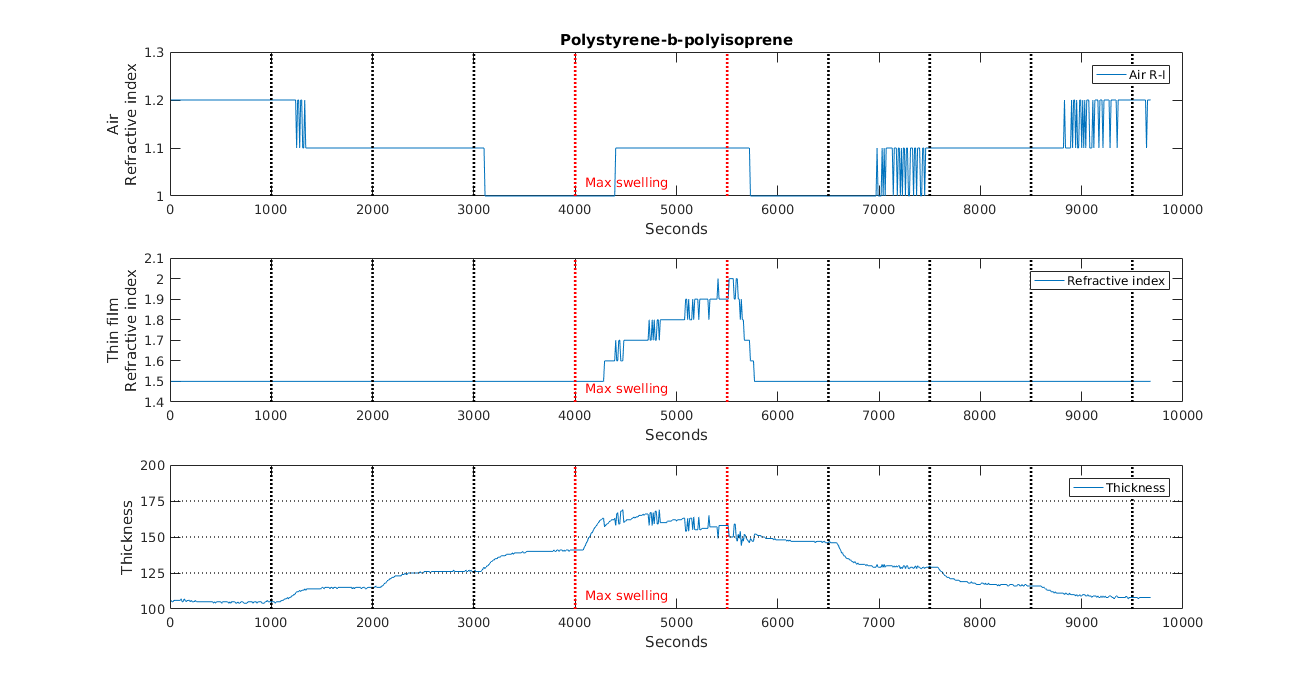
\includegraphics[width=\textwidth]{PSbPIsinglemodel1.png}
\end{frame}

\begin{frame}{Polystyrene-b-polyisoprene MSE}
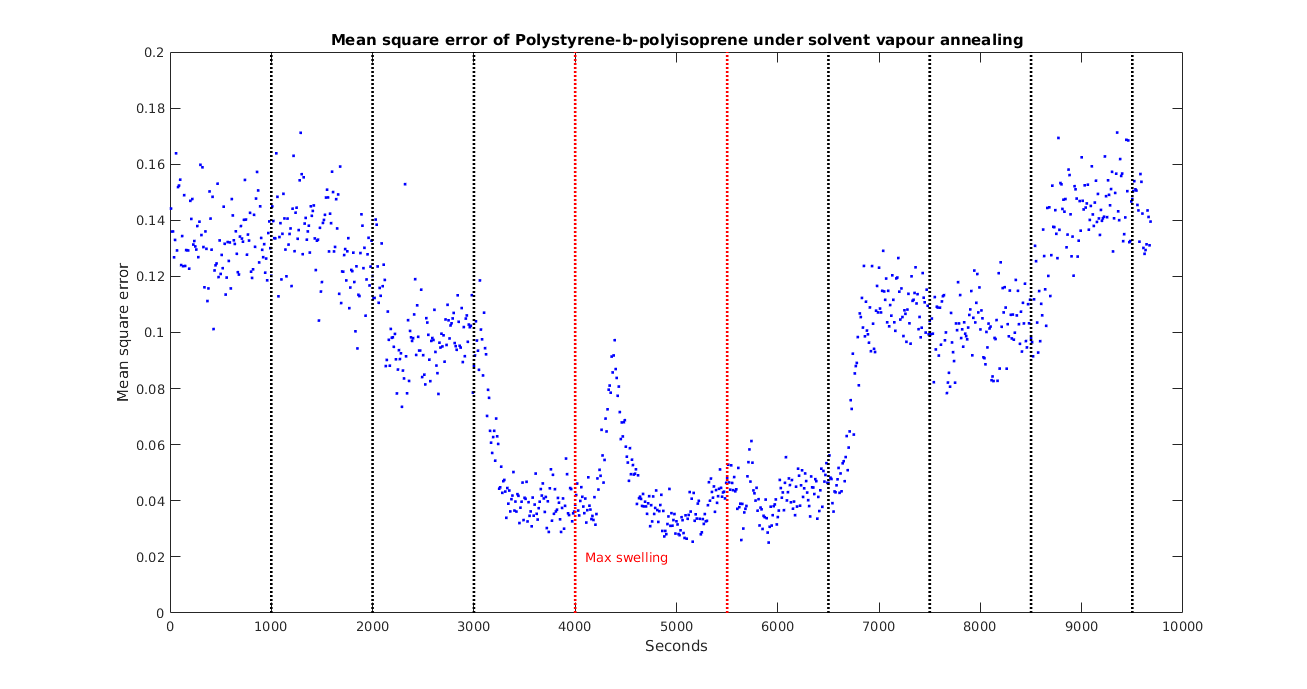
\includegraphics[width=\textwidth]{PSbPIsinglemodel2.png}
\end{frame}

\begin{frame}{Polystyrene-b-polyisoprene comparison}
	\centering
	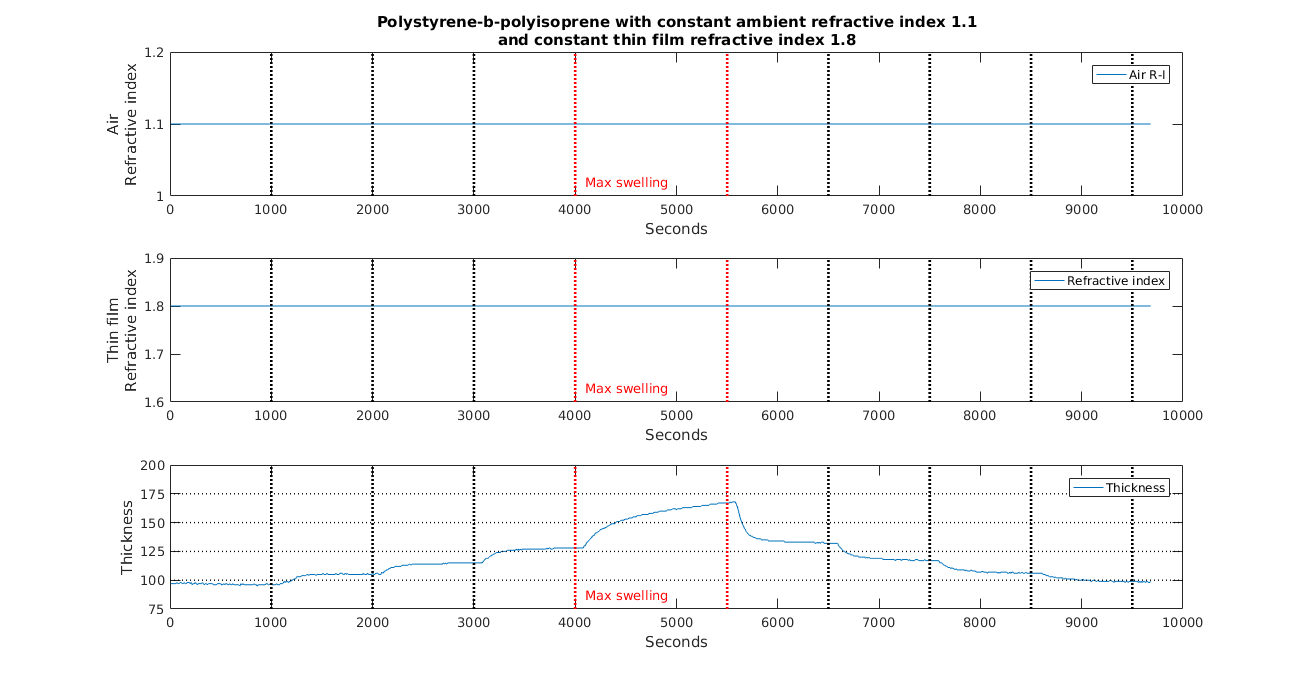
\includegraphics[width=\textwidth]{PSPIn11n18AVG1.png}
\end{frame}

\begin{frame}{Polystyrene-b-polyisoprene comparison}
	\centering
	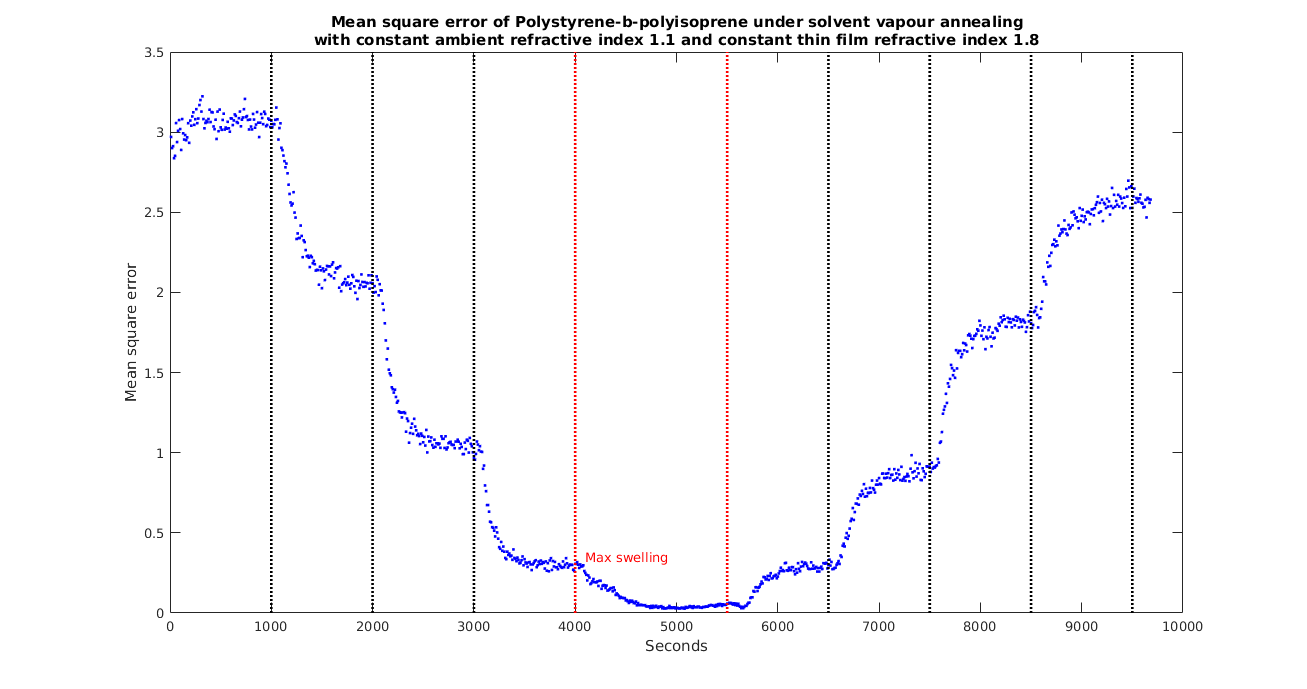
\includegraphics[width=\textwidth]{PSPIn11n18AVG2.png}\
\end{frame}

	\section{Conclusion/Perspective}
	
\begin{frame}{Conclusion/Perspective}

Conclusion:
\begin{itemize}
\item Fresnel equations - easily calculated
\item Care needed when taking dark measurements
\item Light intensity decreases
\item Homopolymer Fresnel model seems optimal for Polystyrene and Polyisoprene but not Polystyrene-b-polyisoprene  
\end{itemize}
Perspective:
\begin{itemize}
\item Refractive index during SVA - Dispersion
\item Polymer - absorption of light
\item Modelling vapour pressure inside solvent vapour annealing test chamber
\item Implementing fitting for multiple layer systems
\end{itemize}

\end{frame}

	\section{Results - 2 polymer layers}
	
\begin{frame}{PS-b-PI}
\begin{center}
	\huge Movie: PSbPIfit2layermodelV2.avi
\end{center}
\end{frame}

\begin{frame}{PS-b-PI - 2 layer model Results}
\centering
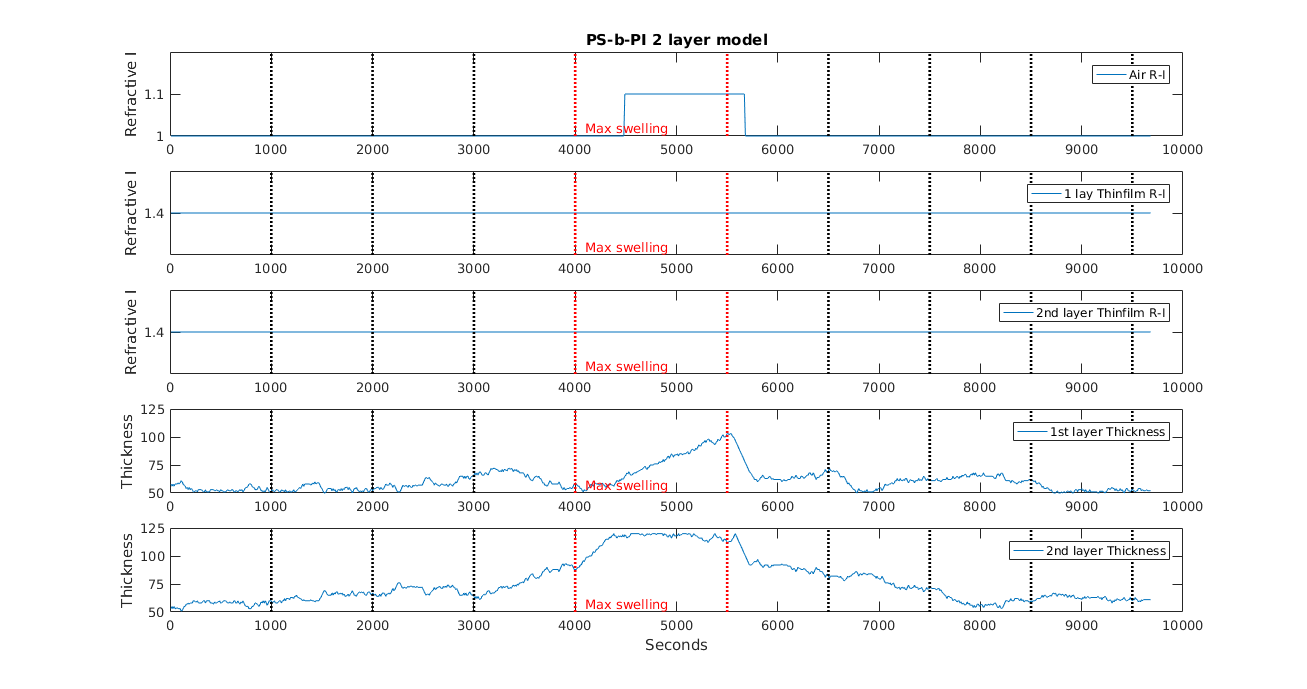
\includegraphics[width=\textwidth]{Results_2layer_PSbPI.png}
\end{frame}

\begin{frame}{PS-b-PI - 2 layer model MSE}
\centering
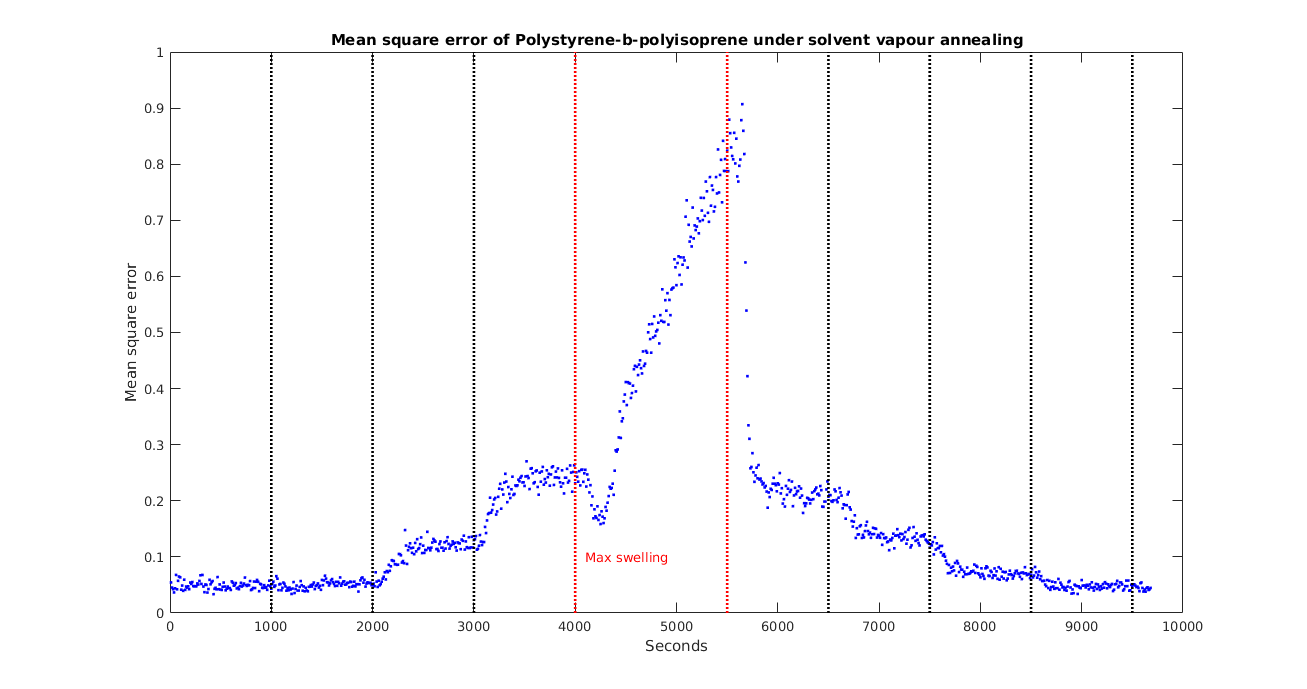
\includegraphics[width=\textwidth]{MSE_2layer_PSbPI.png}
\end{frame}

\begin{frame}{PS-b-PI - 2 layer model total thickness}
\centering
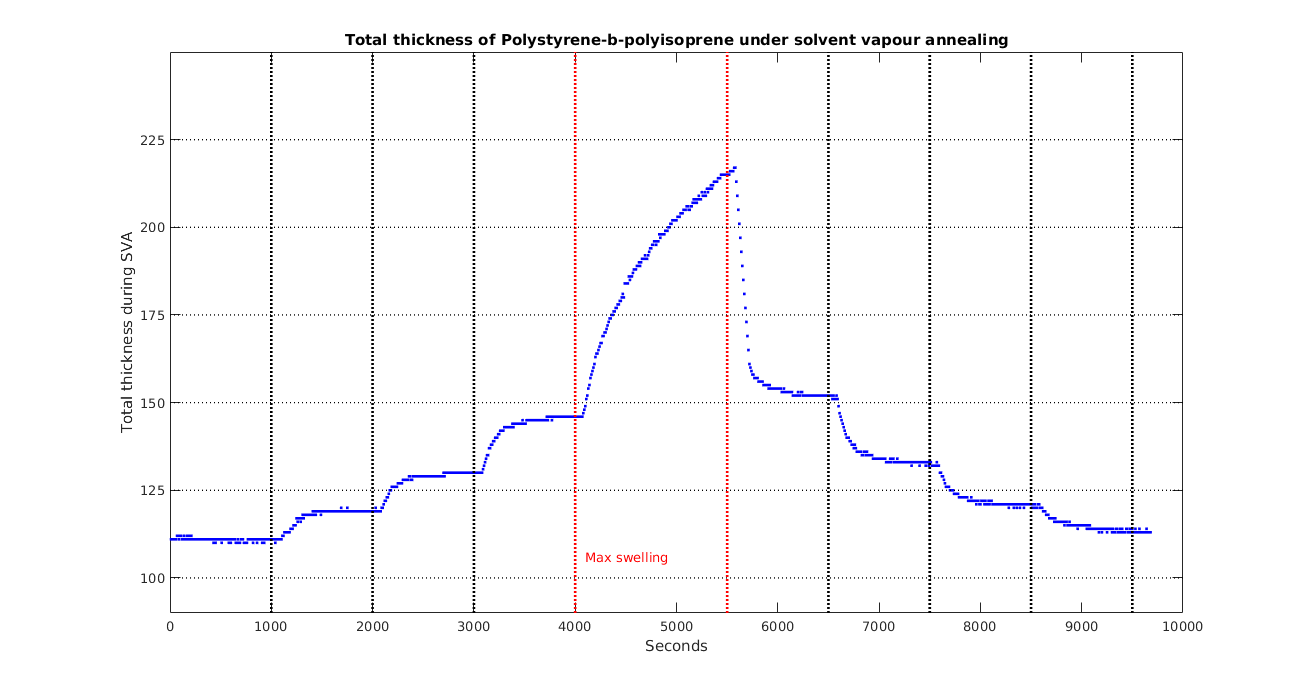
\includegraphics[width=\textwidth]{total_thickness_2layer_PSbPI.png}
\end{frame}

%\begin{frame}{}
%\begin{columns}[t]
%\column{.5\textwidth}
%\centering
%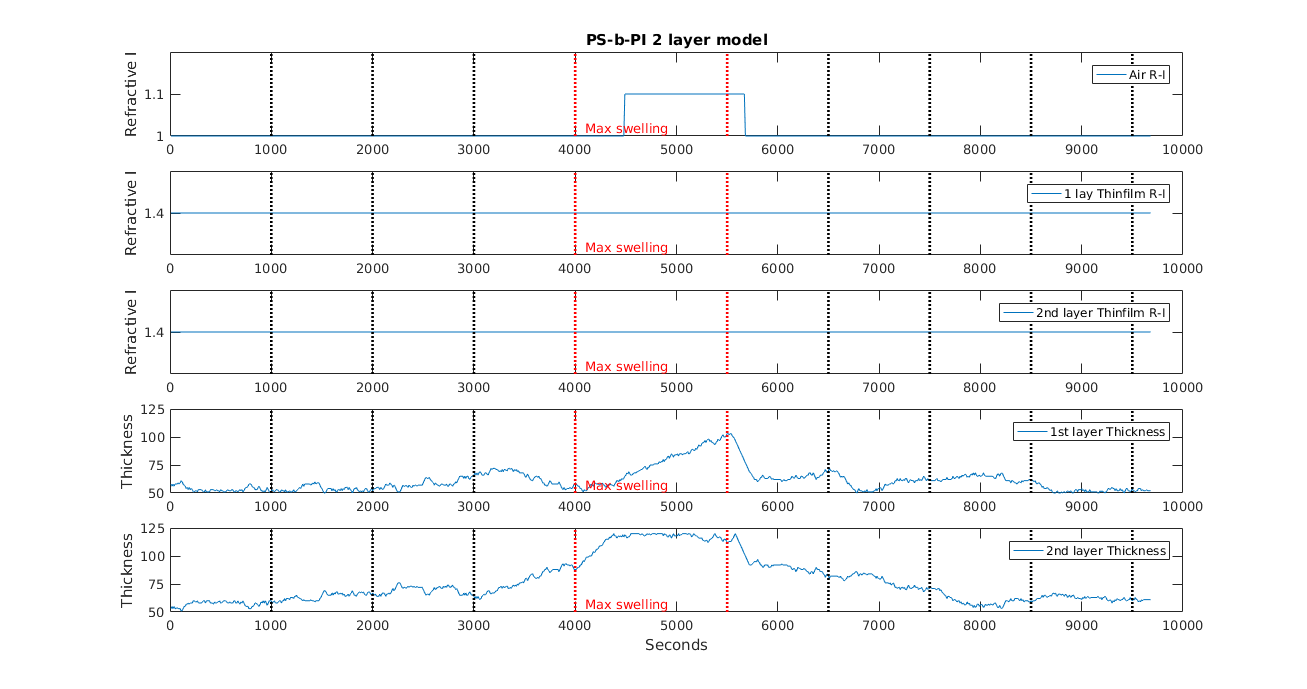
\includegraphics[width=5cm,height=3.5cm]{Results_2layer_PSbPI.png}\\
%\column{.5\textwidth}
%\centering
%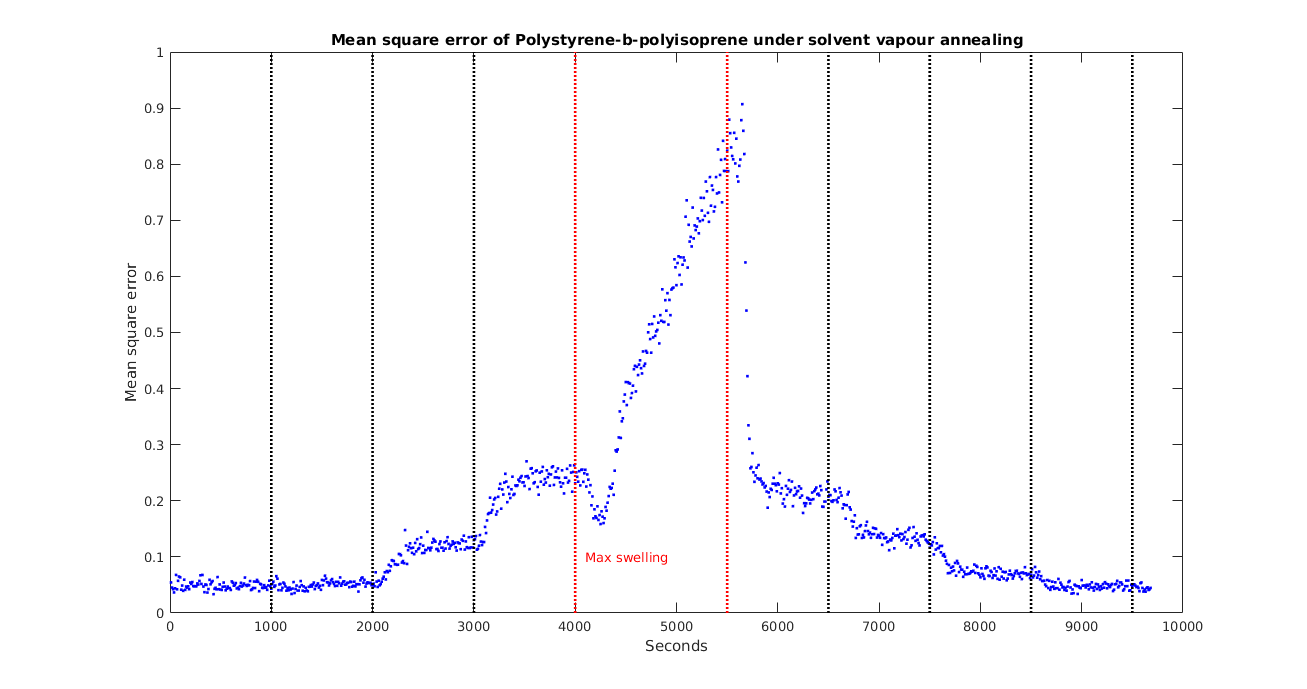
\includegraphics[width=5cm,height=4cm]{MSE_2layer_PSbPI.png}\\
%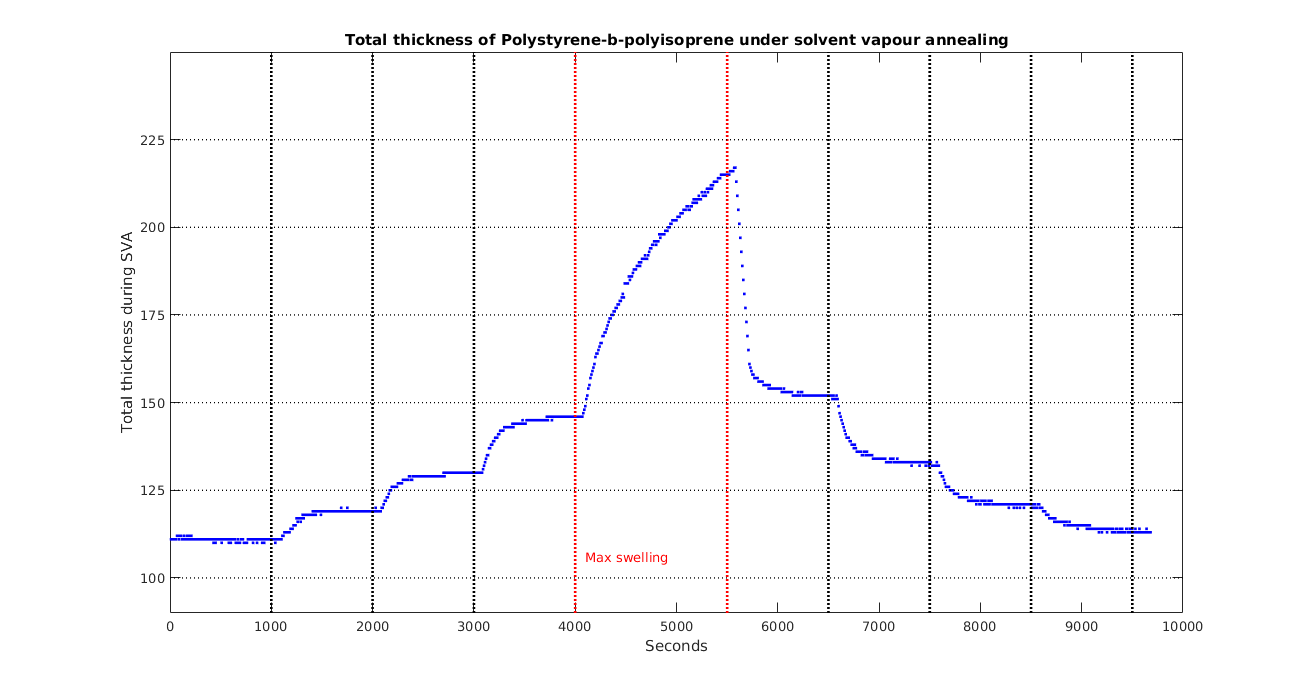
\includegraphics[width=5cm,height=3.5cm]{total_thickness_2layer_PSbPI.png}
%\end{columns}
%\end{frame}

\begin{frame}{PS-b-PI - 2 layer model Results}
\centering
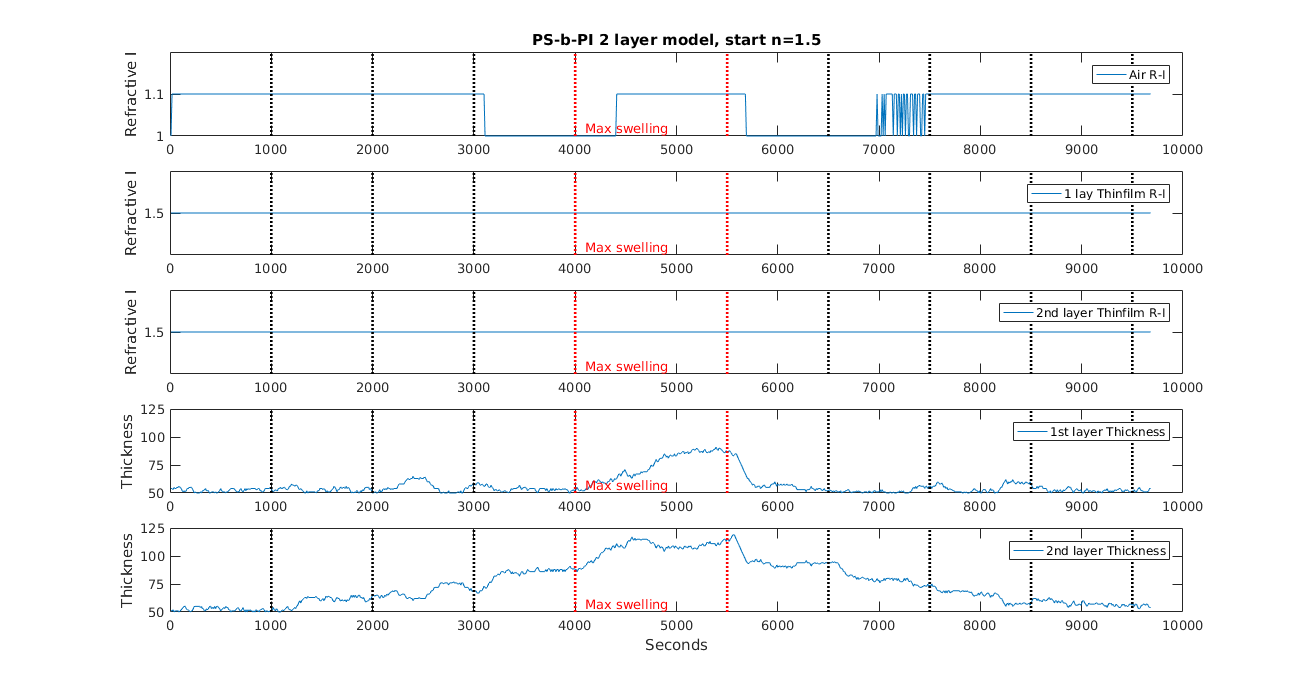
\includegraphics[width=\textwidth]{Results_2layer_PSbPI_n15.png}
\end{frame}

\begin{frame}{PS-b-PI - 2 layer model MSE}
\centering
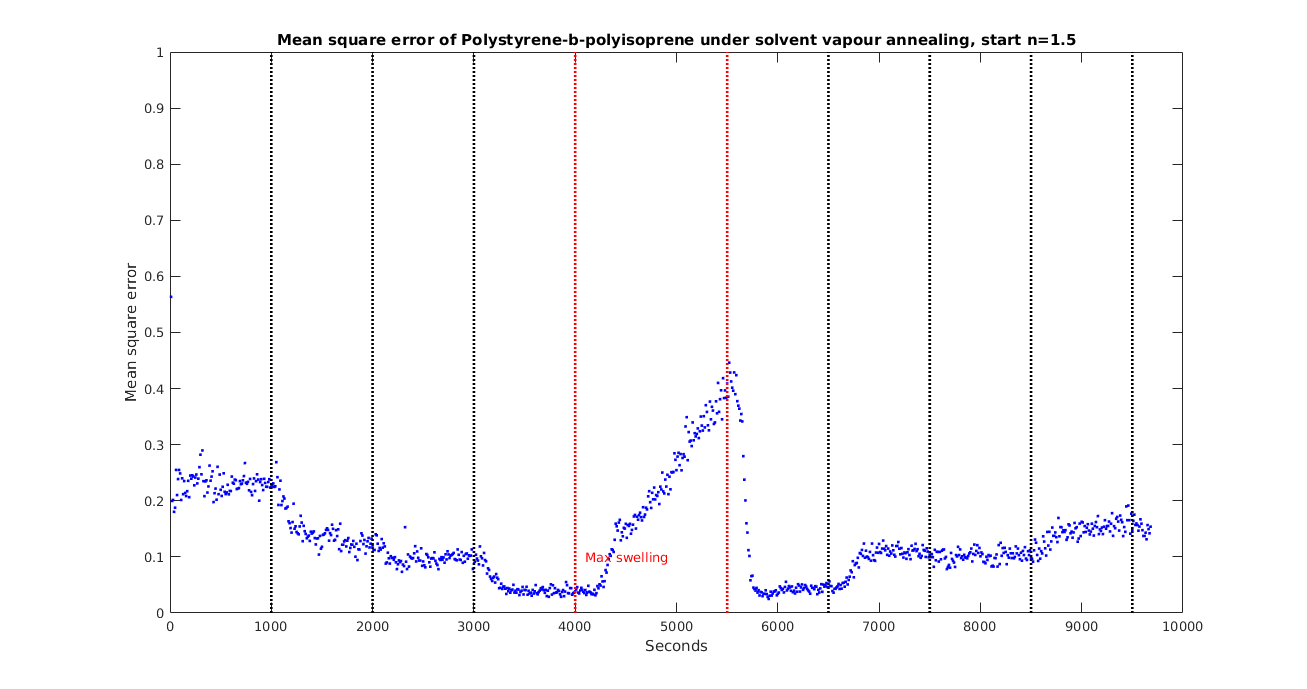
\includegraphics[width=\textwidth]{MSE_2layer_PSbPI_n15.png}
\end{frame}

\begin{frame}{PS-b-PI - 2 layer model total thickness}
\centering
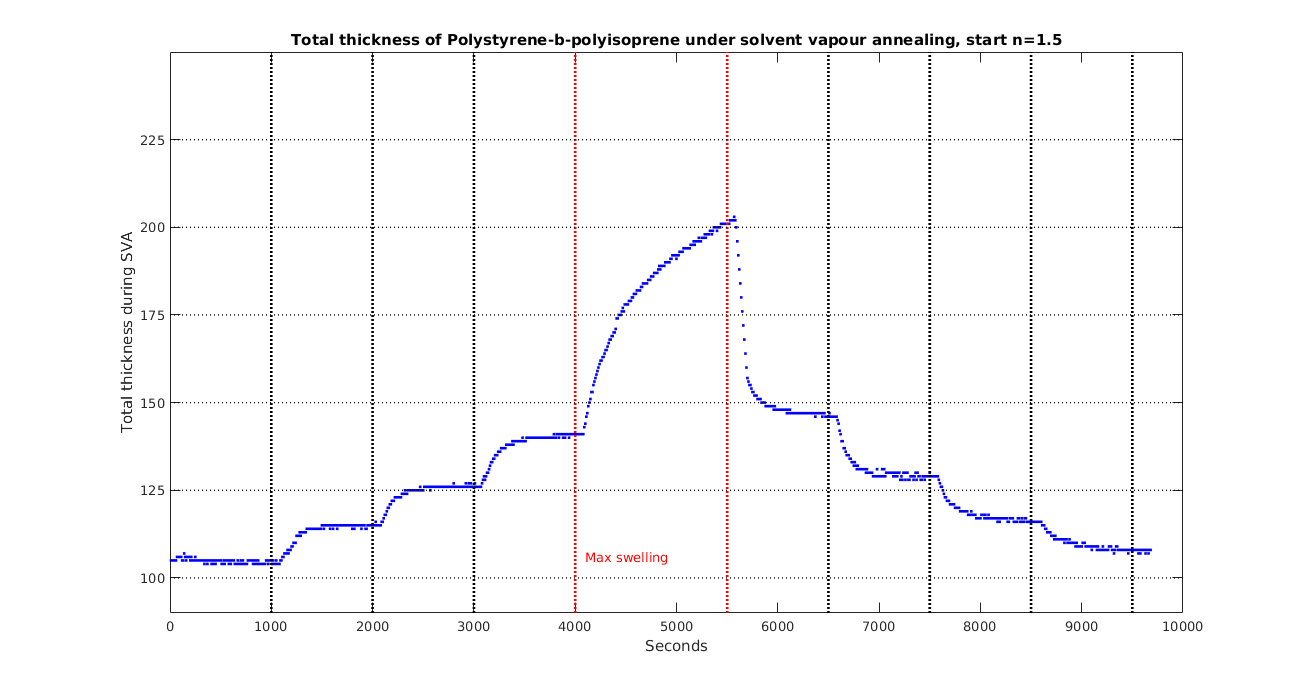
\includegraphics[width=\textwidth]{total_thickness_2layer_PSbPI_n15.png}
\end{frame}

%\begin{frame}{PS-b-PI - 2 layer model}
%\begin{columns}[t]
%	\column{.5\textwidth}
%	\centering
%	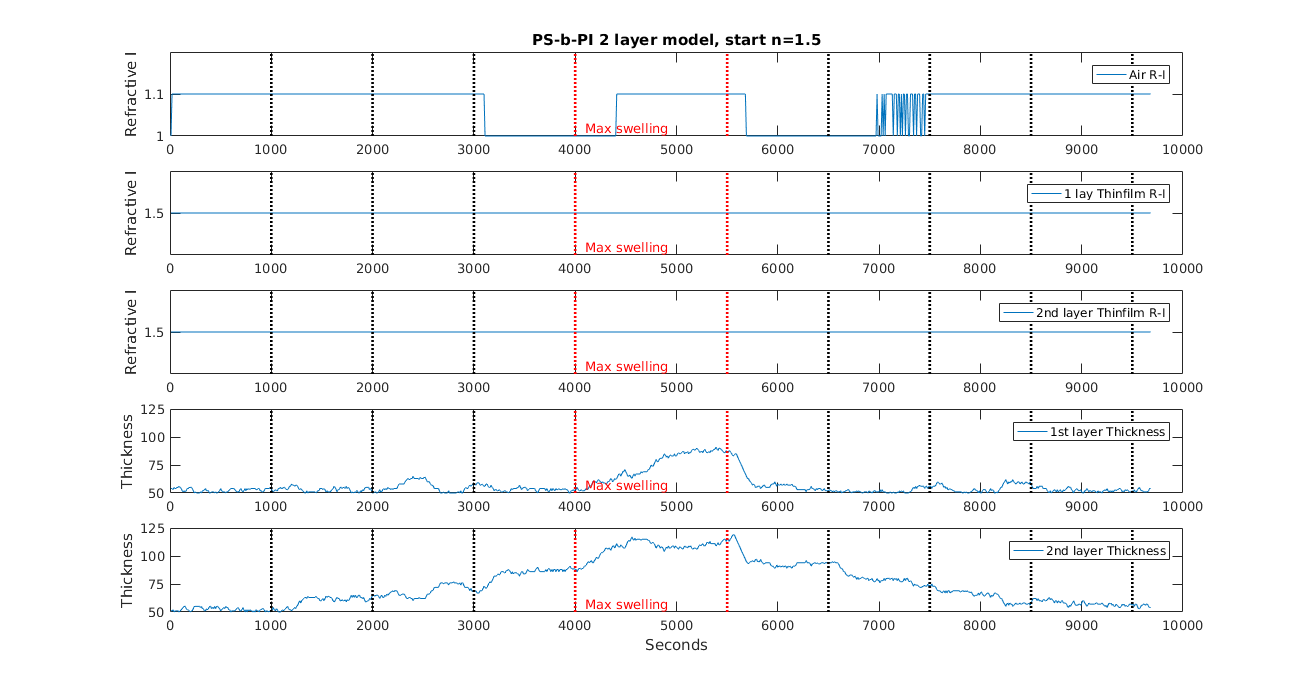
\includegraphics[width=5cm,height=3.5cm]{Results_2layer_PSbPI_n15.png}\\
%	\column{.5\textwidth}
%	\centering
%	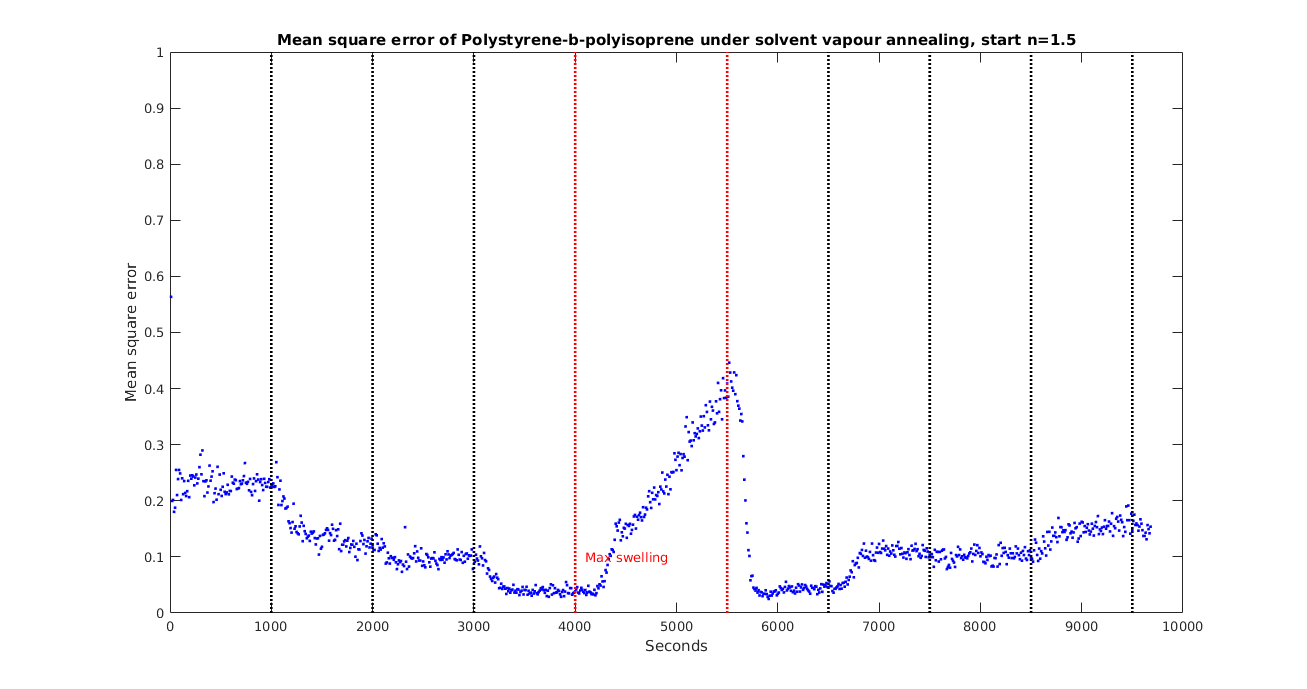
\includegraphics[width=5cm,height=4cm]{MSE_2layer_PSbPI_n15.png}\\
%	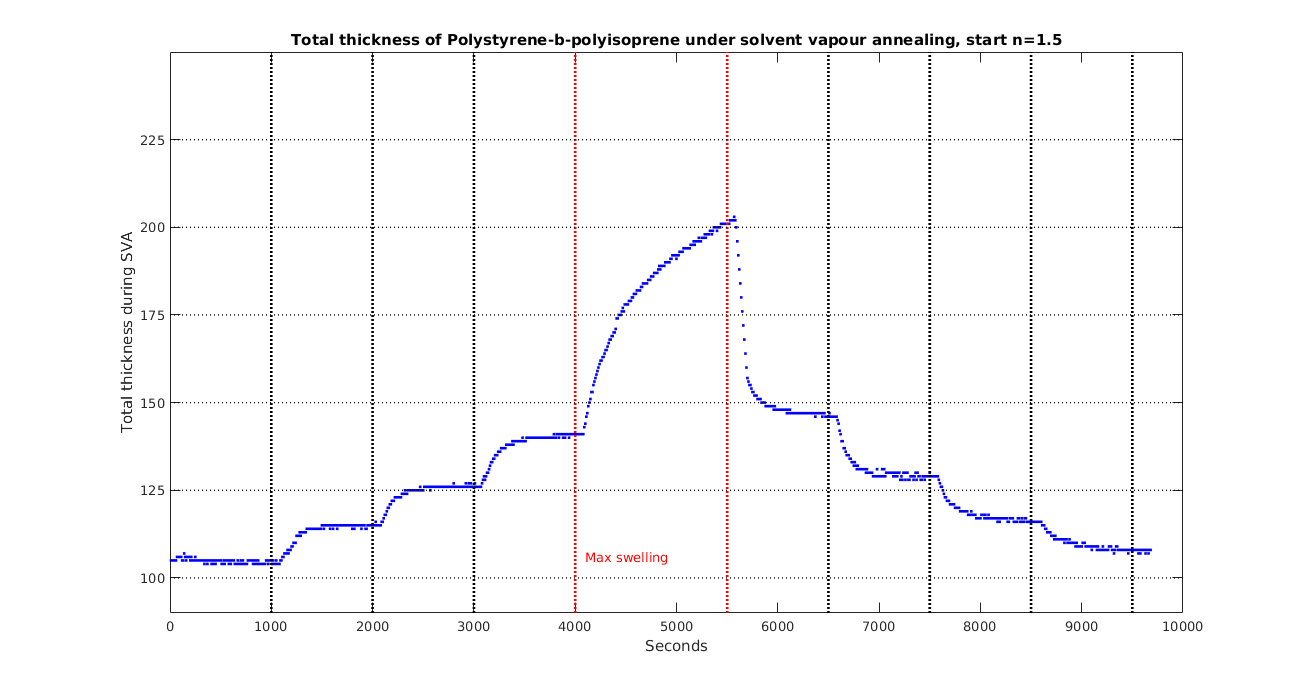
\includegraphics[width=5cm,height=3.5cm]{total_thickness_2layer_PSbPI_n15.png}
%\end{columns}
%\end{frame}
	






%  OLD SLIDES
%
%
%	
%	\begin{frame}{Fresnel equations - multilayers}
%	
%	\begin{figure}
%	\centering
%	\begin{minipage}{0.5\textwidth}
%	\centering
%	\includegraphics[scale=0.2]{figmulti1re.png}
%	\end{minipage}\quad
%	\begin{minipage}{0.5\textwidth}
%	\begin{figure}
%	\centering
%	\includegraphics[scale=0.2]{figmulti2re.png}
%	\end{figure}
%	\end{minipage}
%	\end{figure}
%	
%	\end{frame}
%	
%	\begin{frame}{Fresnel equations - multilayers Cont.}
%	
%	\begin{minipage}{0.47\textwidth}
%	\begin{equation*}
%	r_{123}= \frac{r_{12}+r_{23}\exp(-i2\beta_2)}{1+r_{12}r_{23}\exp(-i2\beta_2)}
%	\end{equation*}
%	
%	\begin{equation*}
%	r_{0123}= \frac{r_{01}+r_{123}\exp(-i2\beta_1)}{1+r_{01}r_{123}\exp(-i2\beta_1)}
%	\end{equation*}
%	\end{minipage}
%	\begin{minipage}{0.5\textwidth}
%		\begin{equation*}
%		\beta=\frac{2\pi d}{\lambda} n\cos(\theta)
%		\end{equation*}
%	\end{minipage}
%	\end{frame}
	
%	\begin{frame}{Polymer refractive index dispersion}
%	Cauchy empirical equation for the refractive index in the visible light range.
%	
%	\begin{equation*}
%	n(\lambda) = A + \frac{B}{\lambda^2} + \frac{C}{\lambda^4}
%	\end{equation*}
%	
%	These constants can be found using ellipsometry.
%	
%	Which dispersion to use? Can Cauchy be used for more exotic polymers?   
%	\end{frame}
%	\section{Preliminary Results}
%	
%	\begin{frame}{Substrate Results}
%		\begin{figure}
%		\centering
%		\includegraphics[width=\textwidth]{sub1.png}
%		\end{figure}
%		\end{frame}
%		
%		\begin{frame}{Substrate Results}
%			\begin{figure}
%			\centering
%			\includegraphics[width=\textwidth]{sub2.png}
%			\end{figure}
%			\end{frame}
%			
%			\begin{frame}{Substrate Results}
%						\begin{figure}
%						\centering
%						\includegraphics[width=\textwidth]{topsil.png}
%						\end{figure}
%						\end{frame}
%						
%		\begin{frame}{Dark and Ref of Topsil in the test chamber}
%		\begin{figure}
%		\centering
%		\includegraphics[scale=0.35]{darkref1.png}
%		\end{figure}
%		\end{frame}
%		\begin{frame}{Dark and Ref of Topsil in the test chamber}
%		\begin{figure}
%		\centering
%		\includegraphics[scale=0.35]{darkref2.png}
%		\end{figure}
%		\end{frame}
%	
%		\begin{frame}{Polystyrene Results}
%			\begin{figure}
%			\centering
%			\includegraphics[width=\textwidth]{p1.png}
%			\end{figure}
%			\end{frame}
%	
%	\begin{frame}{Polystyrene Results}
%		\begin{figure}
%		\centering
%		\includegraphics[width=\textwidth]{p2.png}
%		\end{figure}
%	\end{frame}
%	
%	\begin{frame}{Polystyrene Results}
%		\begin{figure}
%		\centering
%		\includegraphics[width=\textwidth]{p3.png}
%		\end{figure}
%		\end{frame}
%		
%		\begin{frame}{Isoprene Results}
%				\begin{figure}
%				\centering
%				\includegraphics[width=\textwidth]{i1.png}
%				\end{figure}
%				\end{frame}
%				
%\begin{frame}{Isoprene Results}
%\begin{figure}
%\centering
%\includegraphics[width=\textwidth]{i2.png}
%\end{figure}
%\end{frame}
%
%\begin{frame}{Isoprene Results}
%\begin{figure}
%\centering
%\includegraphics[width=\textwidth]{i3.png}
%\end{figure}
%\end{frame}
%
%\begin{frame}{Methyl Methacrylate Results}
%\begin{figure}
%\centering
%\includegraphics[width=\textwidth]{m1.png}
%\end{figure}
%\end{frame}
%
%\begin{frame}{Methyl Methacrylate Results}
%\begin{figure}
%\centering
%\includegraphics[width=\textwidth]{m2.png}
%\end{figure}
%\end{frame}
%
%\begin{frame}{Methyl Methacrylate Results}
%\begin{figure}
%\centering
%\includegraphics[width=\textwidth]{m3.png}
%\end{figure}
%\end{frame}
%
%\begin{frame}{Future plans}
%\begin{itemize}
%\item Tools to analyse reflectance curves.
%\item Model the lens in test chamber setup.
%\item Refine the experimental protocol.
%\item Investigate the polymers.
%\item Begin to investigate diblock polymers.
%\item Begin to investigate other options for modelling the polymers.
%\end{itemize}
%
%\begin{figure}
%\centering
%\includegraphics[scale = 0.2]{differentmodels.png}
%\end{figure}
%\end{frame}





\end{document}